% !TeX encoding = UTF-8
% !TeX spellcheck = fr_FR
% !TeX root = ../mythesis.tex
% !TeX program = pdflatex (build)
%%% TeXmaker : no 'magic comments' but set Root with Options > Set as master file

%useful stuff for what follows

\setcounter{topnumber}{2}
\setcounter{bottomnumber}{0}
\setcounter{totalnumber}{2}
\renewcommand{\topfraction}{0.99}
\renewcommand{\textfraction}{0.01}
\renewcommand{\floatpagefraction}{0.8}

\graphicspath{{./}{./fig/}{./chap_custom_st/fig/}}

\chapter{Optical generation and spectroscopy of arbitrary acoustic horizons}

\label{chap:generation_transonic_fluid}


The previous chapter showed that the creation of a sonic horizon in a polariton fluid can lead to spontaneous emission of Bogoliubov modes provided the downstream region exhibits a collective excitation spectrum with
negative energy modes. Furthermore, it was shown that the strength of the emitted signal depends strongly on the curvature of the horizon, or in other words, its steepness. To ensure that such effect is in principle observable in the laboratory, one needs to fully characterize the mean field of the fluid and locally probe its excitation spectrum. This chapter is dedicated to the description of the full optical generation of arbitrary transcritical fluids as well as the characterization of the excitation spectrum on both sides of the horizon. 
This measurement revealed for the first time negative energy modes in a supersonic quantum fluid, validating the possibility to observe particle creation in a polariton fluid.

The first part of the chapter will focus on the generation of mean fields with arbitrary velocity profiles through the shaping of the pump laser phase. In the second part, we will present the pump-probe spectroscopy method used to locally measure the collective excitation spectrum, as well
as the results obtained for several transonic fluids with different parameters. The results obtained are reported in \cite{falque2024polaritonfluidsquantumfield}.

\section{Optical generation of an arbitrary fluid velocity field}


Set the coordinates $x$ and $y$ to describe the microcavity plane. As explained in \autoref{chap:polariton_theory}, translational invariance in the $xy$-plane ensure in-plane momentum conservation along photon absorption, while the wavevectors along the
$z$ direction are fixed by the cavity and quantum well lengths. Furthermore, in this experiment, the laser beam is set to be quasi-resonant with the lower polariton branch. As a consequence, the transverse phase of the laser is directly imprinted on the polariton field.
Indeed, in the low wavevector limit, the lower polariton branch can be safely approximated by a parabola, namely :

\begin{equation}
    \omega_{LP}(\kbf) = \omega_{LP}^0 + \dfrac{\hbar k^2}{2m_{LP}}.
\end{equation}

The group velocity of a polariton is then $\vbf = \frac{\partial \omega_{LP}}{\partial k} = \frac{\hbar \kbf}{m_{LP}}= \frac{\hbar \kbf_p}{m_{LP}}$ where $\kp$ is the in-plane wavevector of the pump laser.
In the case of a plane wave we can write $\kp=\vec{\nabla}\theta(\rbf)$ where $\theta(r)$ is the spatial phase. This can safely be generalized to more complex spatial phase profiles,
which provides a direct link between the driving laser phase and the velocity of the fluid :

\begin{equation}
    \vbf = \dfrac{\hbar \vec{\nabla} \theta(\rbf)}{m_{LP}} .
\end{equation}

\subsection{Waterfall configuration}
A first realization of a 1D acoustic black hole in a polaritonic system was done in \cite{nguyen_acoustic_2015} with the so-called waterfall configuration. 
The setup was composed of a microcavity etched to be one-dimensional (a microwire), and a defect was added in the middle of the wire to act as an external attractive potential and force the polariton flow to accelerate. The pump was only shone in the region upstream of the defect. The downstream region of the flow was then made of polaritons that propagate ballistically and whose speed is fixed by the interaction energy
in the upstream region.
Even though this configuration provides a natural fluid acceleration, the horizon geometry depends strongly on the defect shape and cannot be tuned easily.  Furthermore, the collective excitation spectrum and the presence of negative energy modes were not investigated, which 
prevented from concluding on the nature of the signal observed in the experiment. In this chapter, we present a different approach to generate such flows with an effective 1D fluid fully optically created, as well as a full characterization of the Bogoliubov spectrum.

\subsection{Target velocity profile}
Before analyzing whether the fluid exceeds a critical velocity, the primary objective is to generate a flow exhibiting two homogeneous regions separated by a sharp transition, each characterized by a well-defined velocity. For clarity, the region preceding the transition will be referred to as the upstream region, with velocity $v_{up}$ while the region following the transition will be designated as the downstream region, with velocity $v_{d}$.
To model this configuration, a target velocity profile is arbitrarily defined as follows:
\begin{equation}
    v(x)= \frac{v_{d}-v_{up}}{2}\mathrm{tanh}(\frac{x-x_h}{w_h})+\frac{v_{up}+v_{d}}{2}
    \label{eq:target_velocity}
\end{equation}
where $x_h$ and $w_h$ are the position and width of the transition respectively. This profile is represented in \autoref{fig:target_velocity.pdf} \textbf{a)}.
One can then verify that :

\begin{subequations}
    \begin{align}
    &\lim\limits_{x-x_h\ll-w_h} v(x) = v_{up},\\
    &\lim\limits_{x-x_h\gg+w_h} v(x) = v_{d}.
    \end{align}
\end{subequations}

\begin{figure}[h]
    \centering
    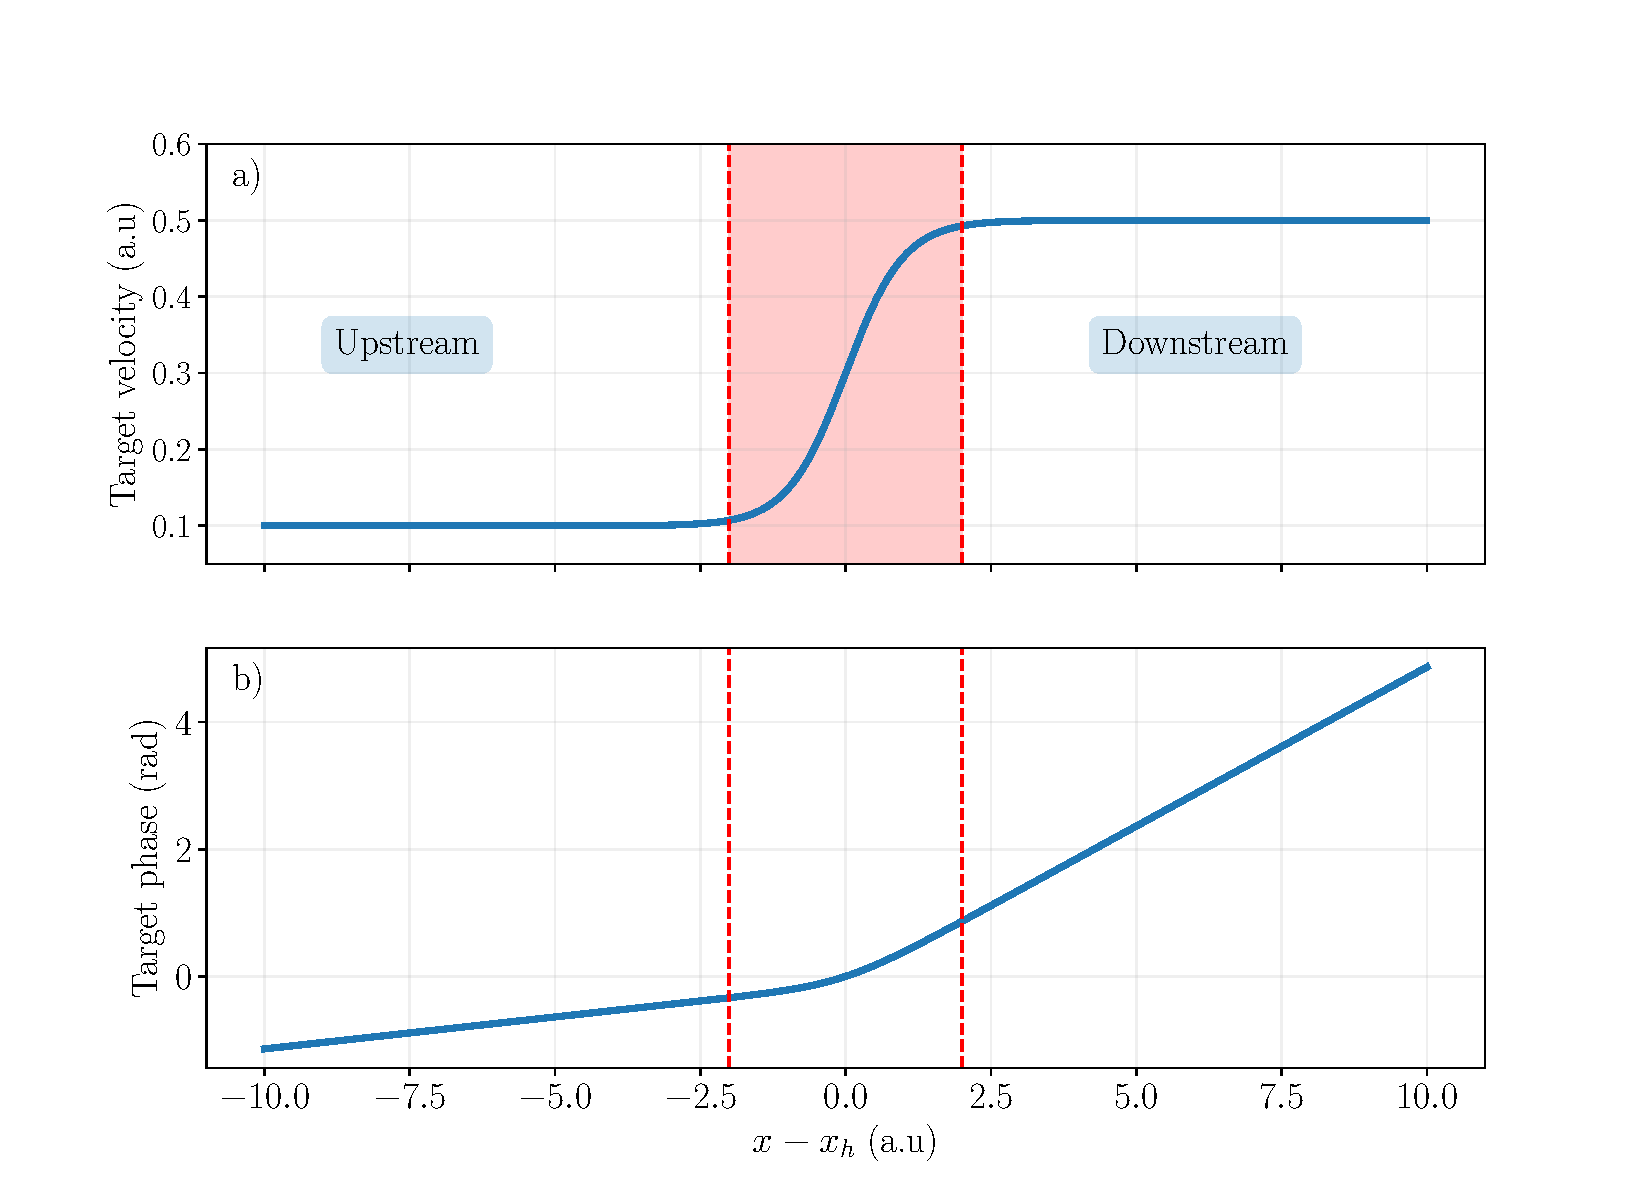
\includegraphics[width=1\textwidth]{chap_custom_st/fig/target_velocity.pdf}
    \caption{ \textbf{a)} Target velocity profile for input parameters $v_{up}=0.1$, $v_{d}=0.5$, $x_h=0$ and $w_h=1$ in arbitrary units. The red shaded area represent the 
    transition region. \textbf{b)} Corresponding phase profile to be imprinted on the pump laser.}
    \label{fig:target_velocity.pdf}
\end{figure}

Such a velocity profile provides great flexibility in the choice of the upstream and downstream velocities as well as the steepness and the position of the transition. From this, one can determine the phase that must be imprinted on the pump laser to generate such a flow profile by simple integration of \autoref{eq:target_velocity}, which gives :

\begin{equation}
    \phi(x) = \dfrac{m_{LP}}{\hbar} \int v(x) dx = \dfrac{m_{LP}}{\hbar} \left( \dfrac{v_{d}-v_{up}}{2} w_h \mathrm{ln}(\cosh(\dfrac{x-x_h}{w_h}))+\dfrac{v_{up}+v_{d}}{2}x \right).
    \label{eq:target_phase_profile}
\end{equation}
The latter is plotted in \autoref{fig:target_velocity.pdf} \textbf{b)}. The derivative of this curve at the position $x$ corresponds to the local wavevector of the pump laser, or equivalently, this curve provides a cut of the wavefront of the driving laser.
 Indeed, the wavefront is defined as the surface of constant phase of the beam. Notably, considering that the driving laser also possesses a wavevector along the $z$ direction, determined by the resonance conditions, the isophase surfaces of the total laser phase $\theta_{laser}$ are given by:  

\begin{equation}
    \begin{aligned}
    \theta_{laser}(r)&=k_zz+\phi(x)=cst \\
                      &=\frac{2\pi n_{cav} }{\lambda_0}z+\theta(x)= cst,
    \end{aligned}
\end{equation}

which is inverted as $z\propto \phi(x)$. Making a fluid with the desired velocity field then reduces to be able to imprint the phase \autoref{eq:target_phase_profile} on the laser that resonantly excites the fluid. As we will see in the next section, this can be done with a Spatial Light Modulator (SLM). 

 A simplified scheme showing how the printing of the target wavefront in the sample plane creates the desired flow is presented in \autoref{fig:wavefront_shapping} \textbf{a)}.
To verify that the fluid has the expected phase, we use the off-axis interferometry method whose principle is explained in \autoref{sec:phase_measurement}
As an example, the measured phase corresponding to the mean field displayed in \autoref{fig:wavefront_shapping} \textbf{b)} is shown in \autoref{fig:phase_example}.
 
\begin{figure}
    \centering
    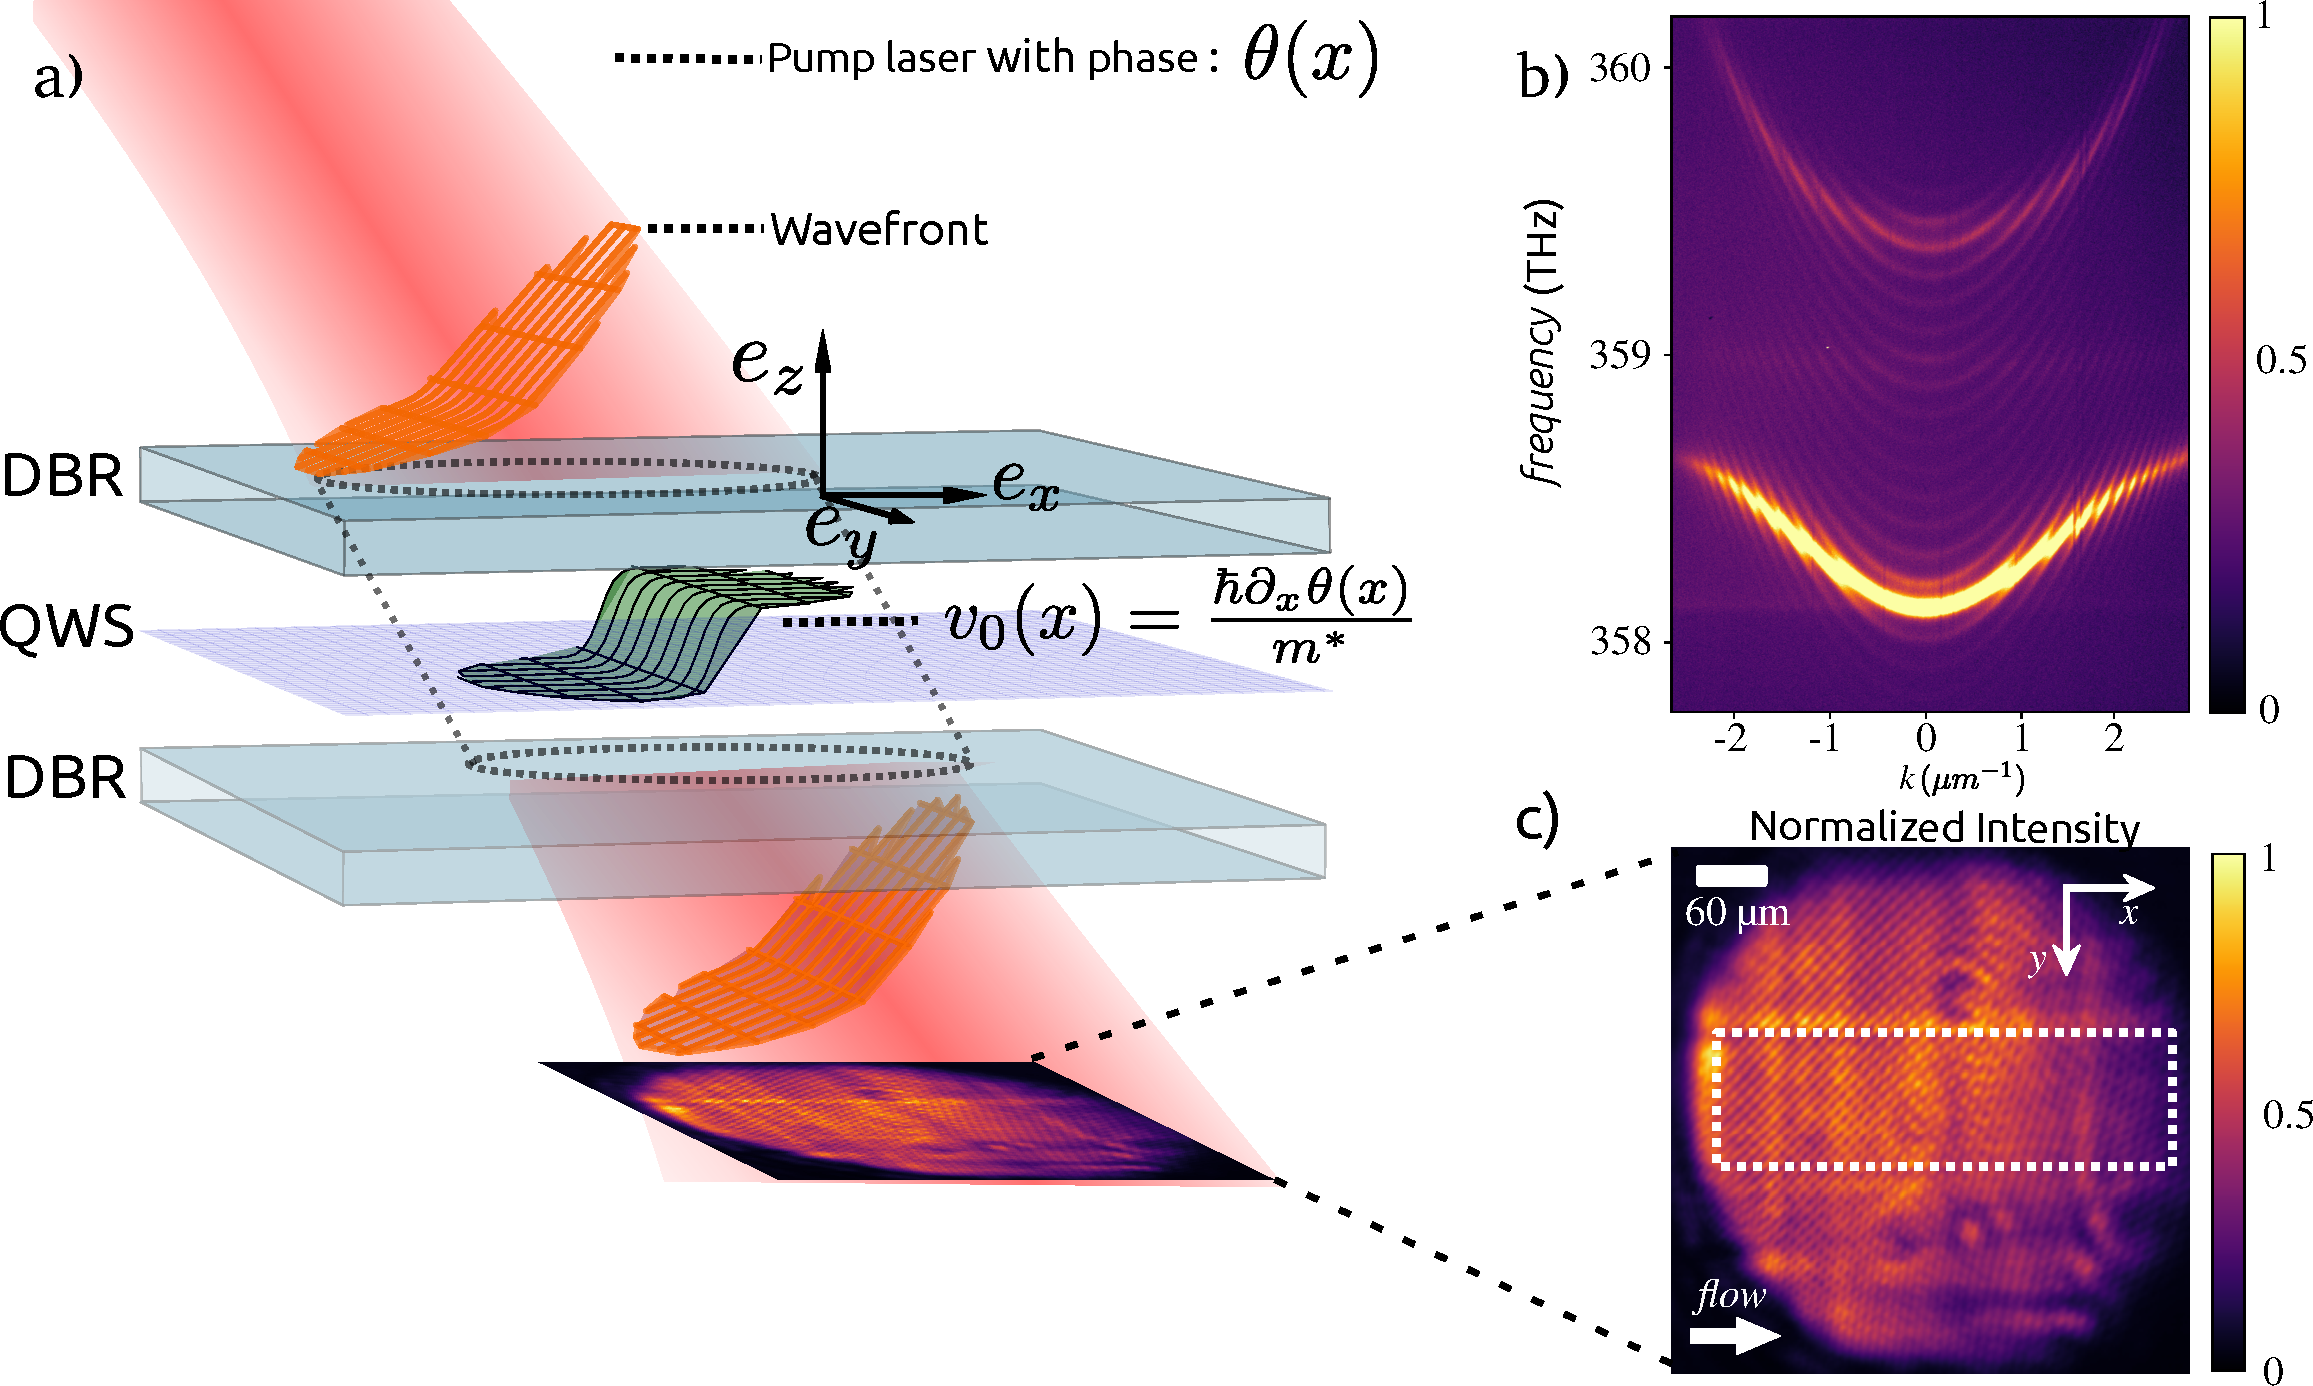
\includegraphics[width=1\textwidth]{chap_custom_st/fig/wavefront_shapping.pdf}
    \caption{Simplified scheme of the generation of a transonic fluid. \textbf{a)} The pump laser is shaped with the target phase profile and sent on the microcavity. The corresponding fluid velocity field is represented by the black surface lying on the Quantum Wells (QWs). c) The outgoing photons are collected and the sample 
    plane is imaged on a CCD camera to obtain the fluid density map.  \textbf{b)} Measured Lower and Upper polariton dispersion at the working point $C6-D6$ at which the experiment was run. By fitting these dispersions,
    the effective LP mass can be extracted $\mlp= 7.0 \times 10^{-35}$ kg}
    \label{fig:wavefront_shapping}
\end{figure}


\bigskip 

\textbf{Controlling the local intensity}. Being able to modify on demand the intensity of the pump laser along with the phase is also crucial since the polariton fluid density, and thus the regime of collective excitations, depends on the input intensity as explained in \autoref{chap:AG_theory}. 
Notably, if the system operates at the turning point of the upper bistability loop, it exhibits a linear collective excitation spectrum, and the speed of sound is directly linked to the detuning of the laser with respect to the lower polariton branch as $gn+g_rn_r=\delta(k_p)$. 
More generally, the possibility to move onto the higher branch of the bistability enables control over the gap opening in the Bogoliubov spectrum, transitioning from a linear, massless spectrum to a parabolic, massive one.  
Once again, this can be achieved using the SLM by locally adjusting the depth of the phase grating under the target phase profile, as explained in \autoref{sec:local_intensity}. This adjustment reduces the number of photons directed into the first diffracted order. This method is widely used to create top-hat intensity profiles and is of significant interest in metrology and cold-atom experiments to minimize systematic effects \cite{top_metrology_2018}.  

\bigskip




To summarize, it is possible to generate and monitor a fluid with arbitrary density and velocity flow by shaping the pump laser both in phase and intensity. We hence have a full optical way to create
effective spacetimes on which we can study the propagation of the collective excitations of the fluid near the transition region.

\subsection{Effective 1D fluid}

So far, the description of the fluid both in velocity and density was one-dimensional despite the fluid is actually a 2D system. This assumption
relies on the fact that the fluid wavefunction is invariant under translation in the $y$ direction in the  region of interest represented by the white dashed rectangle of \autoref{fig:phase_example}. This area is about $130 \mu m$ long and $30-40 \mu m $ large. 
Cuts of both the phase and density in the direction orthogonal to the propagation are shown in \autoref{fig:phase_example} \textbf{b)} and c). Periodic modulations are present because of back reflection on the protection screen of the camera sensor and are present even without passing through the sample. These modulations can be removed
using Fourier filtering which allows to compute the variation of the phase with respect to $2\pi$,  $\sigma_y^{ph}/2\pi$= 0.3\% as well as the relative intensity variation $\sigma_y^I/\langle I \rangle$ =3\%. As a consequence,
we can safely assume that the fluid is effectively 1D in the region of interest. This is in contrast with the work \cite{nguyen_acoustic_2015} previously mentioned. In the present configuration, the shape of the horizon is fixed by the phase of the exciting laser and can be tuned at will, which is crucial to
study the effect of the horizon steepness on the emitted signals. Moreover, the presence of the pump laser in the downstream region brings a significant advantage : the velocity of the fluid can be changed as will and does not depend on the interaction energy of the upstream region, allowing the study of many fluid configurations.


\begin{figure}[h]
    \centering
    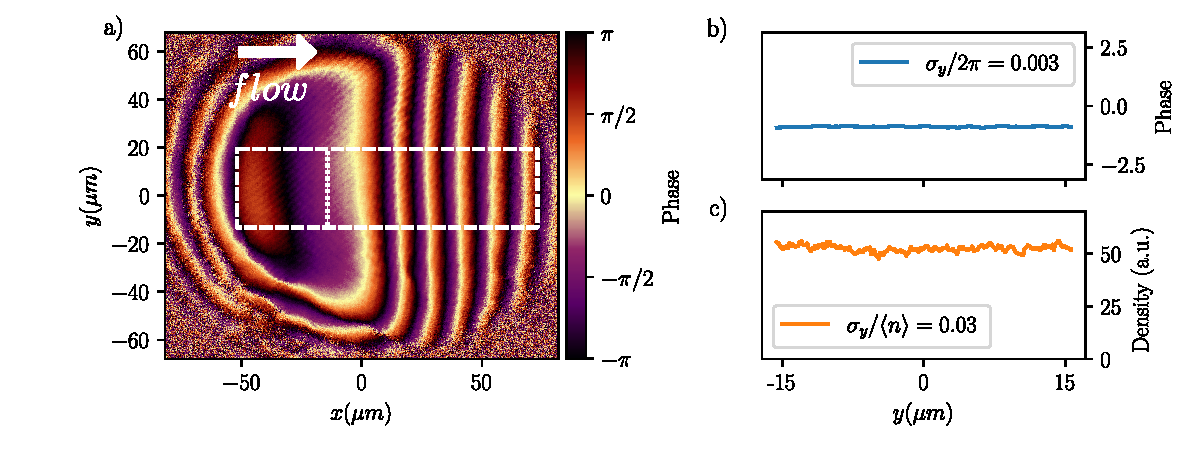
\includegraphics[width=1\textwidth]{chap_custom_st/fig/phase_example.pdf}
    \caption{\textbf{a)} Measured phase of the mean field shown in \autoref{fig:wavefront_shapping}. The curvature present in the upstream region is due to the nonlinear self-focusing. The region
    on interest in which we assume translational invariance is represented by the white dashed rectangle. \textbf{b)}  Cut of the phase in the $y$ direction represented by the dotted white line in the rectangle. The variation to the phase with respect
    to $2\pi$ is equal to 0.3\%. c) Cut of the intensity of the mean field in the $y$ direction at the same location as \textbf{b)}. The corresponding relative intensity variation is equal to 0.3\%.}
    \label{fig:phase_example}
\end{figure}

\section{Experimental spectroscopy of the collective excitation spectrum}

The analog of the Hawking radiation in a polariton fluid is the spontaneous emission of Bogoliubov modes from the horizon. When the system is operating at the turning point of the bistability, the Bogoliubov spectrum 
is gapless and linear which enables the definition of a speed of sound $c_s = \sqrt{\hbar g n /\mlp}$ and speak without ambiguity of sonic excitation in the low wavevector limit. In this regime, the condition to observe negative energy modes coincides with the fluid being supersonic, as explained in the previous chapter. 
However, creating a stable fluid at the turning point is quite challenging and the measurement of the spectrum linearity requires experimental techniques that are hard to implement on a moving fluid \cite{claude_phd}. Nevertheless, linearity is not mandatory to observe Hawking radiation since 
it only requires the mixing between positive and negative energy modes which can be achieved without operating at the turning point. Besides, a gap opening in the Bogoliubov spectrum brings new physics to the table since it widens the study of quasiparticle creation to the case of massive particles. In this
section, we discard the necessity to have sonic excitations and measure the presence of negative energy modes in a wide range of fluid configurations exploring different asymptotic velocities and horizon steepness.

\begin{figure}[h]
    \centering
    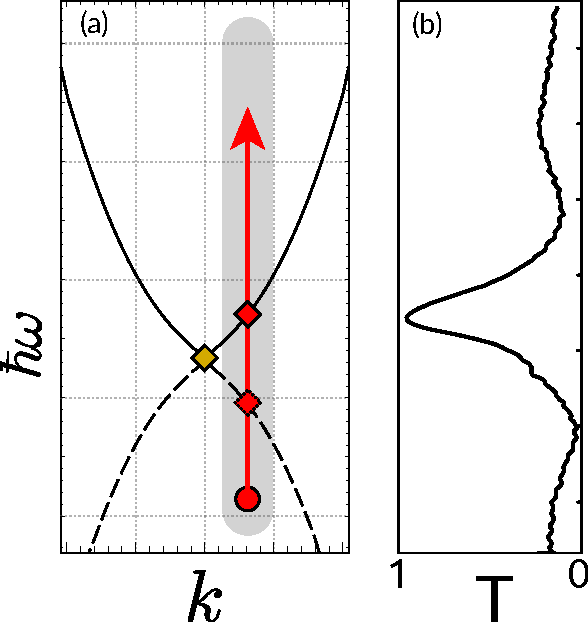
\includegraphics[width=0.3\textwidth]{chap_custom_st/fig/setup_bogoliubov.pdf}
    \caption{Simplified scheme of the pump probe spectroscopy method. \textbf{a)} At a given in plane wavevector represented by the red arrow, the probe frequency is scanned around the mean field frequency and is transmitted when it resonates with the Bogoliubov branch. \textbf{b)} Typical transmission spectrum of the probe at the wavevector of \textbf{a)}.}
    \label{fig:setup_bogo}
\end{figure}


\subsection{High resolution pump-probe spectroscopy method}

\label{sub:high_resolution_spectroscopy}

The measurement of the collective excitations spectrum consists in scanning the mean field resonance by looking at the transmission of a weak probe laser at different incidence angles. First, a polariton fluid is created with a driving laser as described in the previous section. A probe laser is then sent on the sample with a well defined incidence angle corresponding to a precise in plane wavevector, as explained in \autoref{sec:photon}. The frequency of 
the probe is then scanned around the mean field frequency. When the probe frequency matches the frequency of a collective excitation mode, the probe laser gets transmitted by the cavity and can be detected. Frequency scans are then repeated for different incidence angles providing each time a transmission spectrum of the probe as shown in \autoref{fig:setup_bogo}. 
To make sure that we are in the weak perturbation regime the intensity of the probe is set two orders of magnitude below the pump. To collect only the signal emitted in the perturbation mode, a tunable pinhole is placed in the Fourier plane of the collection path and track the probe in-plane wavevector position to filter out the unwanted photons. Finally, the probe intensity is modulated at $f_{mod}$ in order to isolate its transmission from the very strong signal of the pump. The remaining light is then sent on
a photodiode connected to a Spectrum analyzer that demodulates the signal at $f_{mod}$ to obtain the transmission spectrum. At the end, all the scans are put together to reconstruct the full Bogoliubov dispersion as typically shown in \autoref{fig:homogeneous_fluid_bogo}.



\section{Experimental setup}
The setup used in this experiment is shown in \autoref{fig:set_up}. The sample is a microcavity consisting of three InGaAs quantum wells sandwiched between two highly reflecting planar GaAs-AlGaAs Bragg mirrors.
To optimize the light matter coupling, the quantum wells, separated by GaAs barriers, are located at the three antinodes of the cavity, which has a finesse on the order of 3000. A complete map of this sample 
 can be found at the end of this manuscript in \autoref{fig:sample_map} along with exciton-photon detuning measurements. This map enables to perform an experiment over several days at the same working point and overcome the problem due to daily cooling and warming procedures imposed by the open cycle cryostat. Furthermore, despite rigorous and complete
 characterization of the sample, the quality of certain measurements can be substantially enhanced by looking phenomenologically the right working point fitted to the experiment. 
 
 The experiment described in this chapter was run on the working point $C5-D6$.
 The set up is divided in three main paths, the pump path, the probe path and the collection path.


 \begin{itemize}
    \item \textbf{The pump path} represented by the blue box is used to create the steady states of the experiment. The polariton fluid is generated by a circularly polarized CW Ti:sapphire laser with a sub-MHz linewidth. This laser can be precisely frequency tuned around the LP resonance energy centered around 836 nm in our sample. An acusto-optic modulator (AOM) 
    together with a Proportional-integral-derivative feedback on the AOM driving RF are used to stabilize the laser intensity and make sure the experiment is constantly run at a single fluid density.
    The stabilized Gaussian beam is reflected on the spatial light modulator (SLM) which imprints the target phase $\theta_\mathrm{p}(x)=\int v_0(x)dx$ that determines the fluid velocity $v_0(x)$ at each point. The SLM plane is imaged on the input plane of the cavity with two focal-length matched telescopes ($2f-2f$ configuration).
    \item \textbf{The probe path} represented by the red box is used to measure the collective excitation spectrum. The probe is another tunable CW Ti:Sapphire laser with the same polarization than the pump beam. The probe is sent on the sample with a well defined incidence angle controlled by another SLM on which a tunable step blazed grating is imprinted. The frequency of
    the laser is scanned over $\SI{220}{\giga\hertz}$ around the mean field frequency and monitored by a high resolution wavemeter. An AOM and a Proportional-integral-derivative feedback are also used to both stabilize the intensity along the scan and apply a $f_{mod}=\SI{5}{\mega\hertz}$ intensity modulation.
    \item \textbf{The collection path} located after the sample is used to collect the output signals coming from the fluid. A microscope objective sends the outgoing field on a 50:50 BS. One part is directed to an optical system to make the image both in real and momentum space of the field. For both lasers, a pick-up is made after their respective AOM to have a phase reference and perfom off axis interferometry measurement. Another part is sent to the apparatus described in \autoref{sub:high_resolution_spectroscopy} to measure the transmission spectrum of the probe. The tunable
    pinhole is made with a DMD and is placed in the Fourier plan of a lens, selecting only photons arriving at the position of the pinhole and sending them to the collection photodiode. Given 
    the relative size of the probe mode and the size of a pixel of the DMD, the resolution of the pinhole can go down to $\delta k = \SI{0.0005}{\per \micro\meter}$. The collection photodiode is then connected to a spectrum analyzer set in zero span at $f_{mod}$ to demodulated the signal and obtain the transmission spectrum of the probe. On both path
    a set of $\lambda/4,\ \lambda/2$ and $PBS$ allows to control and filter the polarization of the signal.  
 \end{itemize}

 \textbf{Scan resonances analysis.} The maximum value and the linewidth of the probe transmission and reflection peaks are directly related to the real and imaginary parts of the energy $\hbar \ombog$ of the Bogoliubov dispersion relation.
  If we consider plane wave like excitations

\begin{equation}
    \psilp(t) \propto \rmexp (-i \ombog t) = \rmexp \left (- i \re (\ombog) t \right ) \cdot \rmexp \left( \im (\ombog) t \right),
\end{equation}
one easily verifies by taking its temporal Fourier transform that its spectral density has the following Lorentz-distribution law

\begin{equation}
    I(\omega) = \abs{\psilp(\omega)}^2 \propto \dfrac{1}{ \left(\omega - \re(\ombog) \right)^2 + \left( \dfrac{\im(\ombog)}{2} \right)^2}.
\end{equation}

At each probe wavevector $k_{pr}$ the transmission spectrum $I_{k_{pr}}(\omega)$ is fitted with a Lorentzian function to extract the real and imaginary parts of the Bogoliubov dispersion $\ombog(k_{pr})$

 \begin{figure}
    \centering
    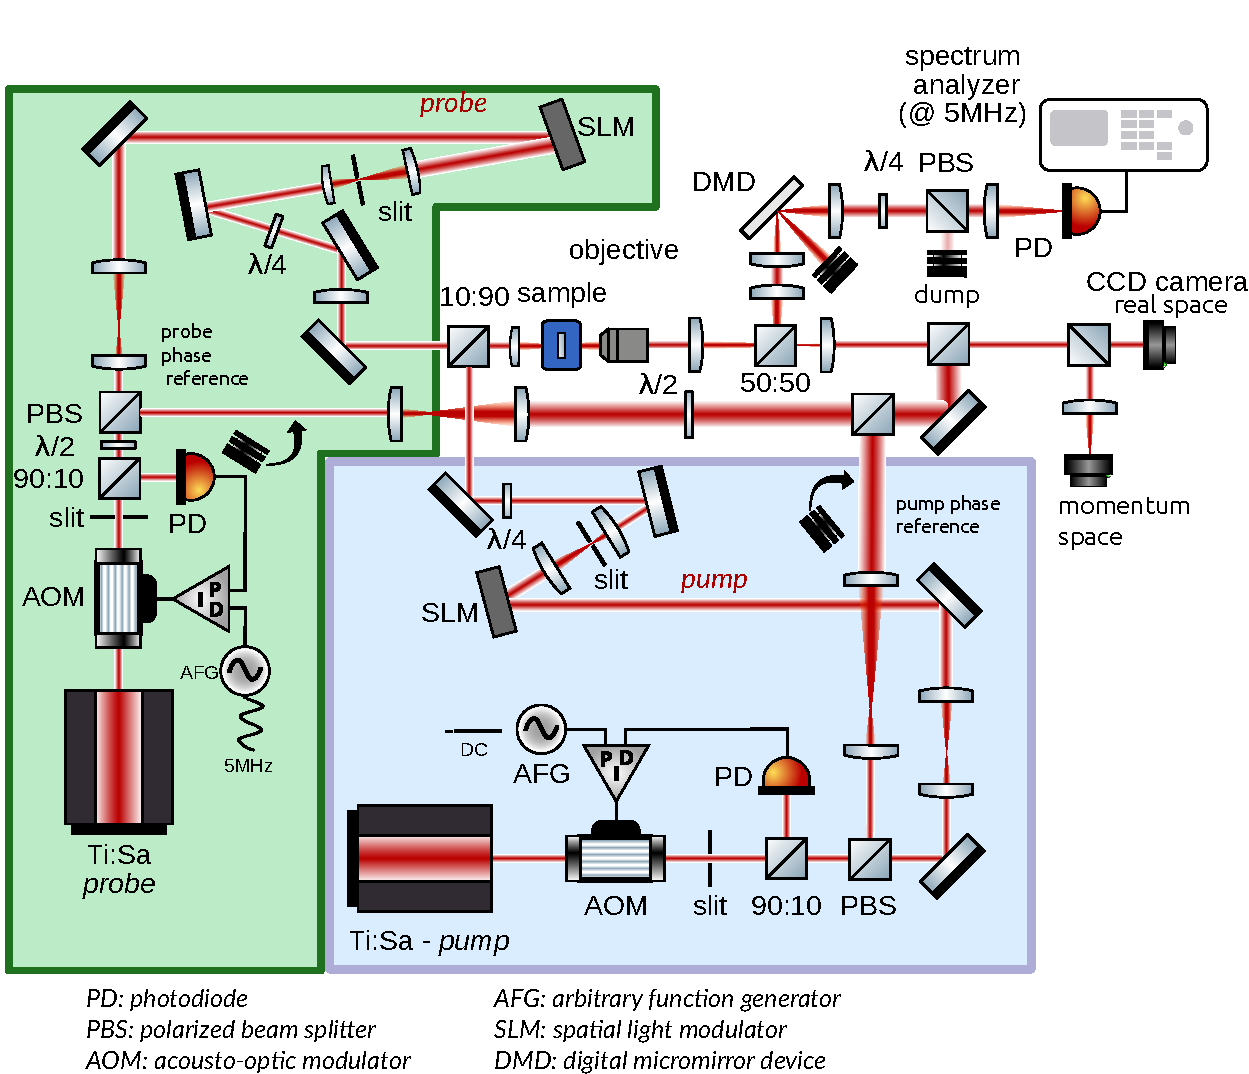
\includegraphics[width=1\textwidth]{chap_custom_st/fig/set_up_spacetime.pdf}
    \caption{Experimental setup}
    \label{fig:setup}
\end{figure}





\section{Experimental results}

\subsection{Homogeneous fluid}

We first study homogeneous fluids with non zero velocities to see the effect of the Doppler shift on the collective excitations spectrum. In this section,
the pump is a gaussian beam which creates fluid having a spatial extension of approximately $150 \ \mathrm{\mu m}$. The input angle of the pump
is controlled in the same way as the probe by printing a tunable step blazed grating on the SLM. In each measurement, the effective detuning 
$\delta(k_p)=\omega_p -\omlp^0- \hbar k_p^2/2\mlp$ is high enough to be in the bistable regime and the input pump intensity is chosen so the system operates on the higher branch of the hystersis curve quite far from the turning point. 
The probe is set to be two order of magnitude weaker than the pump and it has the same spatial extension and polarization.

\bigskip

\textbf{Direct normal branch measurement.} We create a set of homogeneous fluids with increasing in plane wavevectors $k_p$ while keeping the pump frequency constant. 
For each fluid, we use the pump probe spectroscopy method to measure the probe transmission spectrum as shown on \autoref{fig:homogeneous_fluid_bogo}. 
The DMD is programmed to display pinholes that track the wavevector of the probe laser along the scans. In this case the system measures the direct transmission of the probe. The first measurement \textbf{a)} is made with the pump laser turned off which means in the absence of interactions within the sample.
The probe transmission then scan the bare cavity resonances and recover the parabolic shape at low wavevector of LP branch. From this measurement we extract the detuning between the pump laser and the LP branch at zero wavevector
 $\delta(0) = \SI{33}{\giga\hertz}$. 
 The blueshift due to interaction lifts the dispersion \textbf{a)} to higher energies whereas the Doppler shift modifies the resonances according to 
 $\omega' = \omega + \vbf_p\delta \kbf$ where $\vbf_p$ is the fluid velocity $\vbf_p = \hbar \kbf_p/\mlp$.  As the fluid velocity increases, the branch is bended and moved toward the pump wavevector. 
 For $k_p\geq 0.3$ we already see some resonances lying under the pump energy. As explained in the previous chapter, the energy sign of a collective mode is given by :
 
 \begin{equation}
    \mathrm{sign}(E)=\mathrm{sign}(\omega_\mathrm{B})\times \mathrm{sign}(Q_{\phi}),
 \end{equation}
 
where $Q_{\phi}$ is the norm of the mode defined in \autoref{eq:norm} and $\mathrm{sign}(\omega_\mathrm{B})$ is taken with respect to the pump energy. Since the normal branch has a positive norm, the resonances located
below the pump frequency are negative energy modes. As it can be seen, the ghost branch is not visible through direct excitation. This feature has a double origin : first the ghost branch is not optically resonant with the cavity which makes photon injection difficult at its energy. Secondly,
the Bogoliubov coefficient $v_k$ of the negative norm branch is very small compared to $u_k$.  In the presence of
a coherent state like the probe, the populations then scale as $v_k^2 |\alpha|^2\ll u_k^2|\alpha|^2$ where $\alpha$ is the intracavity amplitude of the probe. 

\begin{figure}[h!]
    \centering
    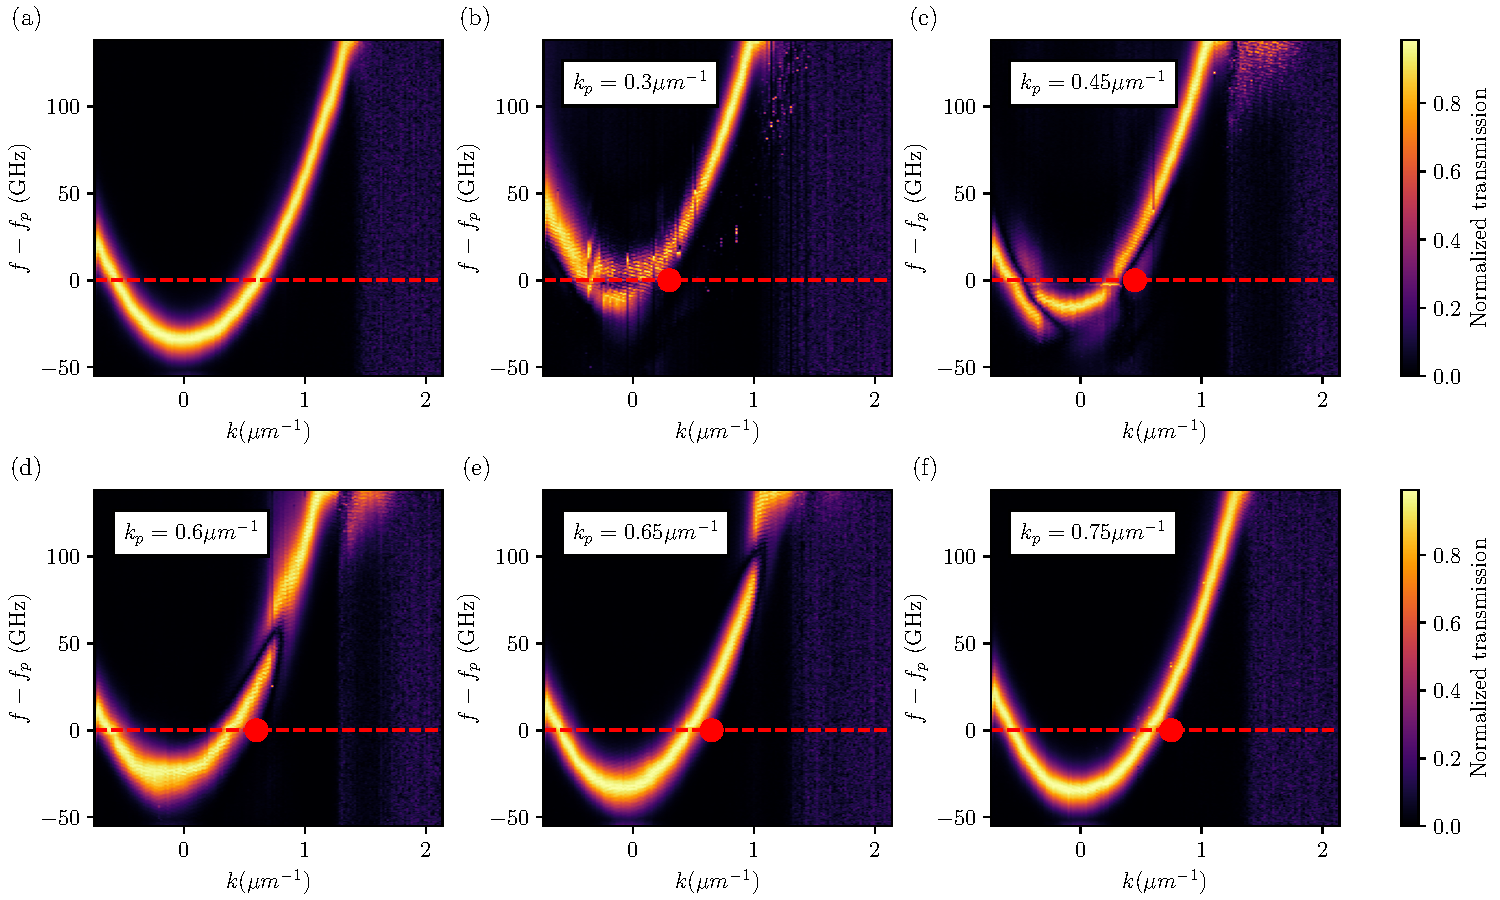
\includegraphics[width=1\textwidth]{chap_custom_st/fig/homogeneous_doppler.pdf}
    \caption{a) Bare cavity dispersion measurement with the pump probe spectroscopy method in the absence of fluid. 
    The parabolic shape of the Lower Polariton branch is observed.  
    The red dashed line represent the mean field frequency that was kept constant for all the measurements. 
    From this we can measure the detuning between the pump laser and the LP branch at $k=0$,
     $\delta(0) = \SI{33}{\giga\hertz}$. \textbf{b)},c),d),e) and f) measured Bogoliubov normal branches for homogeneous fluid with velocities 0.75, 0.98, 1.23, 1.29 and $\SI{1.43}{\micro \meter \per \pico \second}$ respectively, corresponding 
    to the pump wavevector values in the inset of each figure.}
     
    \label{fig:homogeneous_fluid_bogo}
\end{figure}

\bigskip

 \textbf{Ghost branch indirect measurement.} To overcome the difficulty to directly excite the ghost branch, we take advantage of the strong nonlinearities of the system to induce population
 through four wave mixing process. Indeed, because of the bosonic nature of Bogoliubov excitations, the occupation of the normal branch in the probe wavevector mode should stimulate the parametric conversion of two pump polaritons into a Bogoliubov pair with opposite wavevectors and energies with respect to the pump, namely :

 \begin{subequations}
    \begin{align}
    (k_p, k_p) &\rightarrow (k_p+\Delta k, k_p-\Delta k),\\
    (\omega_p, \omega_p) &\rightarrow (\omega_p+\Delta \omega,\omega_p- \Delta \omega).
    \end{align}
 \end{subequations}
The emission in the ghost branch is then boosted by a factor $(u_kv_k)^2|\alpha|^2$ \cite{I_frerot_PRX_2023}. In practice, this measurement
can be done by changing the positions of the tunable pinhole so it tracks wavevectors opposite to the probe with respect to the pump. More precisely,
when a scan at $k_{pr}=k_p+\Delta k$ is made, the pinhole is set at $k_{pr}=k_p-\Delta k$ to collect the signal emitted in the conjugated mode. 

\bigskip

Here we create again a homogeneous fluid with wavevector $k_p =0.6 \mu m^{-1}$. We then 
perform direct measurement of the normal branch and indirect measurement of the ghost branch. The results are shown in \autoref{fig:homogeneous_fluid_bogo_ghost} \textbf{a)} and \textbf{\textbf{b)}} respectively.  The modulations on the right side of the direct measurement come from interferences in the substrate of the sample
that act as a low Q-factor Fabry Perot \cite{claude_phd}. Each scan is normalized to its own maximum for the sake of clarity but 
the strength of the indirect signals is approximatevily $1-10\%$ of the direct one. The noise present on several scan of \textbf{b)} corresponds to parasitic signals coming from other scatterings process that may send photons at the position of the pinhole and that, in the case of direct measurement, are negligible with respect to the resonance. The reason why the ghost branch does not appear as the symmetric of the normal branch 
is because the axis $k$ and $f-f_p$ represents the wavevector and frequency of the injected probe and not the emitted signal. However, the pinhole positions first ensure us that the signal is emitted in the opposite wavector mode. To verify that it is also symmetric in frequency, we send the photons collected through the pinhole 
into a spectrometer to measure their energy. This two tests allox to confirm that the signals taken through indirect measurement in \textbf{\textbf{b)}} indeed come from the ghost branch. As a consequence, it is possible  to symmetrize the indirect data around the pump wavevector and energy to plot the full collective excitation spectrum shown in \autoref{fig:homogeneous_fluid_bogo_ghost} \textbf{c)}. First, one can check that the two branches 
are indeed symmetric with respect to the pump represented by the red dot.
\begin{figure}
    \centering
    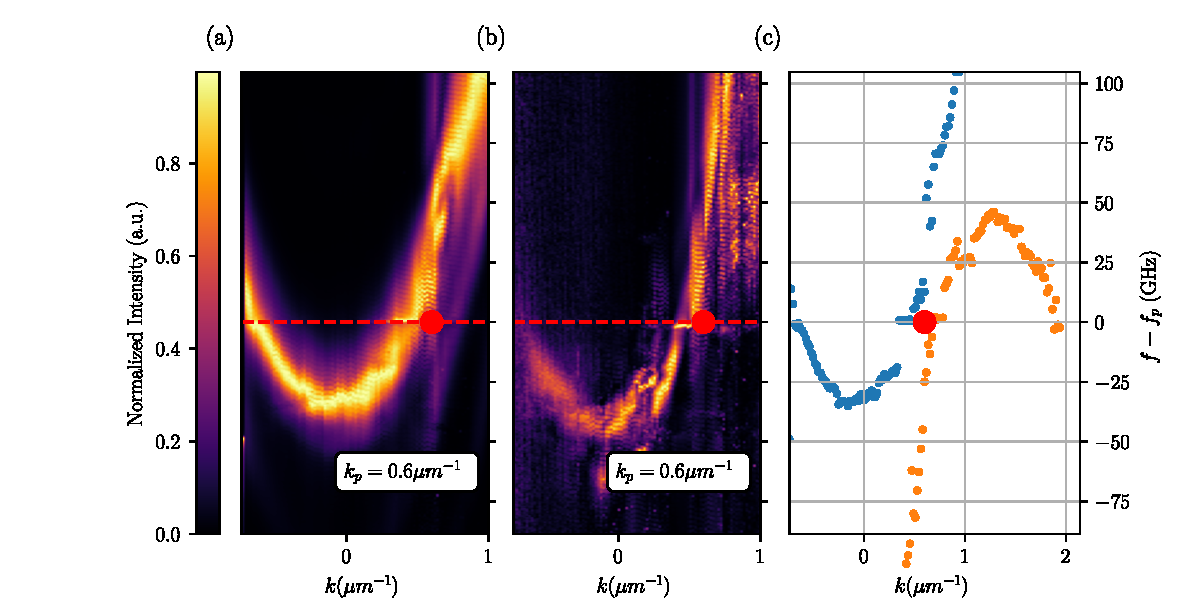
\includegraphics[width=1\textwidth]{chap_custom_st/fig/supersonic_homogenous.pdf}
    \caption{\textbf{a)} Direct measurement of the normal branch of the Bogoliubov spectrum for a homogeneous fluid with in plane wavevector $k_p=\SI{0.6}{\per \micro \meter}.$ \textbf{\textbf{b)}} Indirect measurement of the ghost branch of the Bogoliubov spectrum for the same fluid.
    c) Extracted resonance energy for each probe wavevector. The blue point are extracted from the direct measurement and correspond directly to the resonances of \textbf{a)}. The orange points are extracted from the indirect measurement. Each couple $(k_{pr}, \omega)$ extracted from \textbf{b)} is symmetrized around the pump position in phase space $(k_p, \omega_p)$ to account for FWM process.}
    \label{fig:homogeneous_fluid_bogo_ghost}

\end{figure}

Once again this measurement is an additional proof that for fluid velocities high enough, negative energy modes can be excited on both positive (normal) and negative (ghost) norm branches.
It's worth noticing that no effort were put in this experiment to reach the turning point of the bistability loop which did not prevent the observation of negative energy modes. This relaxes 
the experimental constraints to observe Hawking radiation in a polariton fluid and widens the initial analogy that was made for sonic excitation in a supersonic fluid. More precisely it can be reformulated as follows :
a fluid exhibiting a sharp transition between a region with positive energy modes, and another one with negative energy modes available, should experience  emission of correlated Bogoliubov modes at the transition.
These modes are not necessarily phonons and the velocity to exceed to observe them is not necessarily the speed of sound, but rather a critical velocity that depends more generally on the fluid parameters.
Although this statement seems unclear with respect to the sonic version, it is actually more general and broaden the range of experimental configurations at which particle creation can be observed. In the following 
we will rather speak of trans critical flow and critical velocity instead of "sonic".






\subsection{Smooth transition geometry}

We first study a smooth transition between the sub- and supercritical flow regions.
We implement the target velocity profile \autoref{eq:target_velocity} with a transition width $w_\mathrm{H}=\SI{20}{\micro\meter}$. 
We study three profiles, with three values for the up- and downstream flow velocities $v_\mathrm{u}$ and $v_\mathrm{d}$.
All the measurements are made with $\delta(0)=\SI{56}{\giga\hertz}\rightarrow \hbar\delta(0)= \SI{0.2}{\milli \electronvolt}$.
At this detuning the system is in the bistable regime in both the upstream and downstream regions with a spatial extension of $\SI{120}{\micro \meter}$.
For each configuration, the phase of the created fluid is measured by off-axis interferometry as described in \autoref{sec:phase_measurement}. By unwrapping the phase profile, as the one typically shown in \autoref{fig:smooth_transition} \textbf{a)}, and taking the gradient in the $x$ direction, we obtain the fluid velocity profile $v(x)$.
The measured velocity profiles are represented by the solid lines in \autoref{fig:smooth_transition} \textbf{\textbf{b)}} showing three different asymptotic downstream velocities $v_\mathrm{d}$ with a single upstream velocity $v_\mathrm{u}$. 
To selectively measure the upstream or downstream region the diameter of the probe beam is reduced to half the spatial extension of the fluid and the probe focused on the region of interest. The corresponding excitation spectra are shown in \autoref{fig:smooth_transition} \textbf{c)-f)}. 
The upstream region is shown in \autoref{fig:smooth_transition} \textbf{c)} and the downstream regions in \autoref{fig:smooth_transition} \textbf{d)-f)}.

\bigskip

\subsubsection{Speed of sound measurement} Even though the system does not operate in a regime of sonic collective excitation we call $c_s=\sqrt{\hbar g n/\mlp}$ the speed of sound. The value of $gn$ is extracted 
from the simultaneous fit of the normal and ghost branch of each spectrum with the Bogoliubov dispersion relation :

\begin{equation}
    \label{eq:lfbogo}
    \begin{split}
        \ombog^{\pm}(\delta k)= -\frac{i\gamma}{2}+ v_0(x) \delta k(x)\,\pm \\\sqrt{\left(\frac{\hbar \delta k(x)^2}{2m^*}-\delta(k_p) +2gn(x) +g_\mathrm{r} n_\mathrm{r}    \right)^2-(gn(x))^2},
    \end{split}
\end{equation}
with $\delta k(x)=k-k_p(x)$. The only unkwonw parameters in this equation are $gn$ and $g_rn_r$. However by taking the steady states solution of the Gross Pitaevskii equation coupled to a reservoir \autoref{eq:generalized_GPE} we obtain $n_r\propto n$.
Based on the work \cite{claude_phd,claude_high-resolution_2022} made on the same sample and the assumption that the reservoir contribution depends on the exciton-photon detuning. We use the value $g_rn_r\approx 1.8gn$ of work \cite{claude_phd} and end 
with a single free parameter $gn$ to fit the spectra. The fit are represented by the colored dashed line in \autoref{fig:smooth_transition}. The output of the fit gives in fact a value of $gn(r_{pr})$ where $r_{pr}$ is the position of the probe. However, this value can serve 
as calibration to reconstruct the full $gn(r)$ profile. Indeed we can safely assume that the output measured intensity is proportional to the 
fluid density as $I_{out}(r)=a n(r)$ and that $a$ is a constant that depend on the exciton photon detuning through the hopfield coefficients and complex 
cavity parameters. Nonetheless, given the spatial extension of the fluid with respect to the wedge of the sample $\SI{0.04}{\micro \electronvolt \per \micro \meter}$, these paramateres can be considered as constant in the region of interest.
We can then calibrate the speed of sound measurement through :

\begin{equation}
    \label{eq:speed_of_sound_calib}
    c_\mathrm{s}(r)=\sqrt{\frac{I_{out(r)}}{I_{out}(r_{pr})}}c_s(r_{pr}).
\end{equation}

The $c_s(x)$ map obtained for the different configurations are represented by the dashed lines in \autoref{fig:smooth_transition} \textbf{b)}. The speed of sound is found to be quite constant which yields a smooth transition between the upstream and downstream regions. 

\bigskip

\begin{figure}
    \centering
    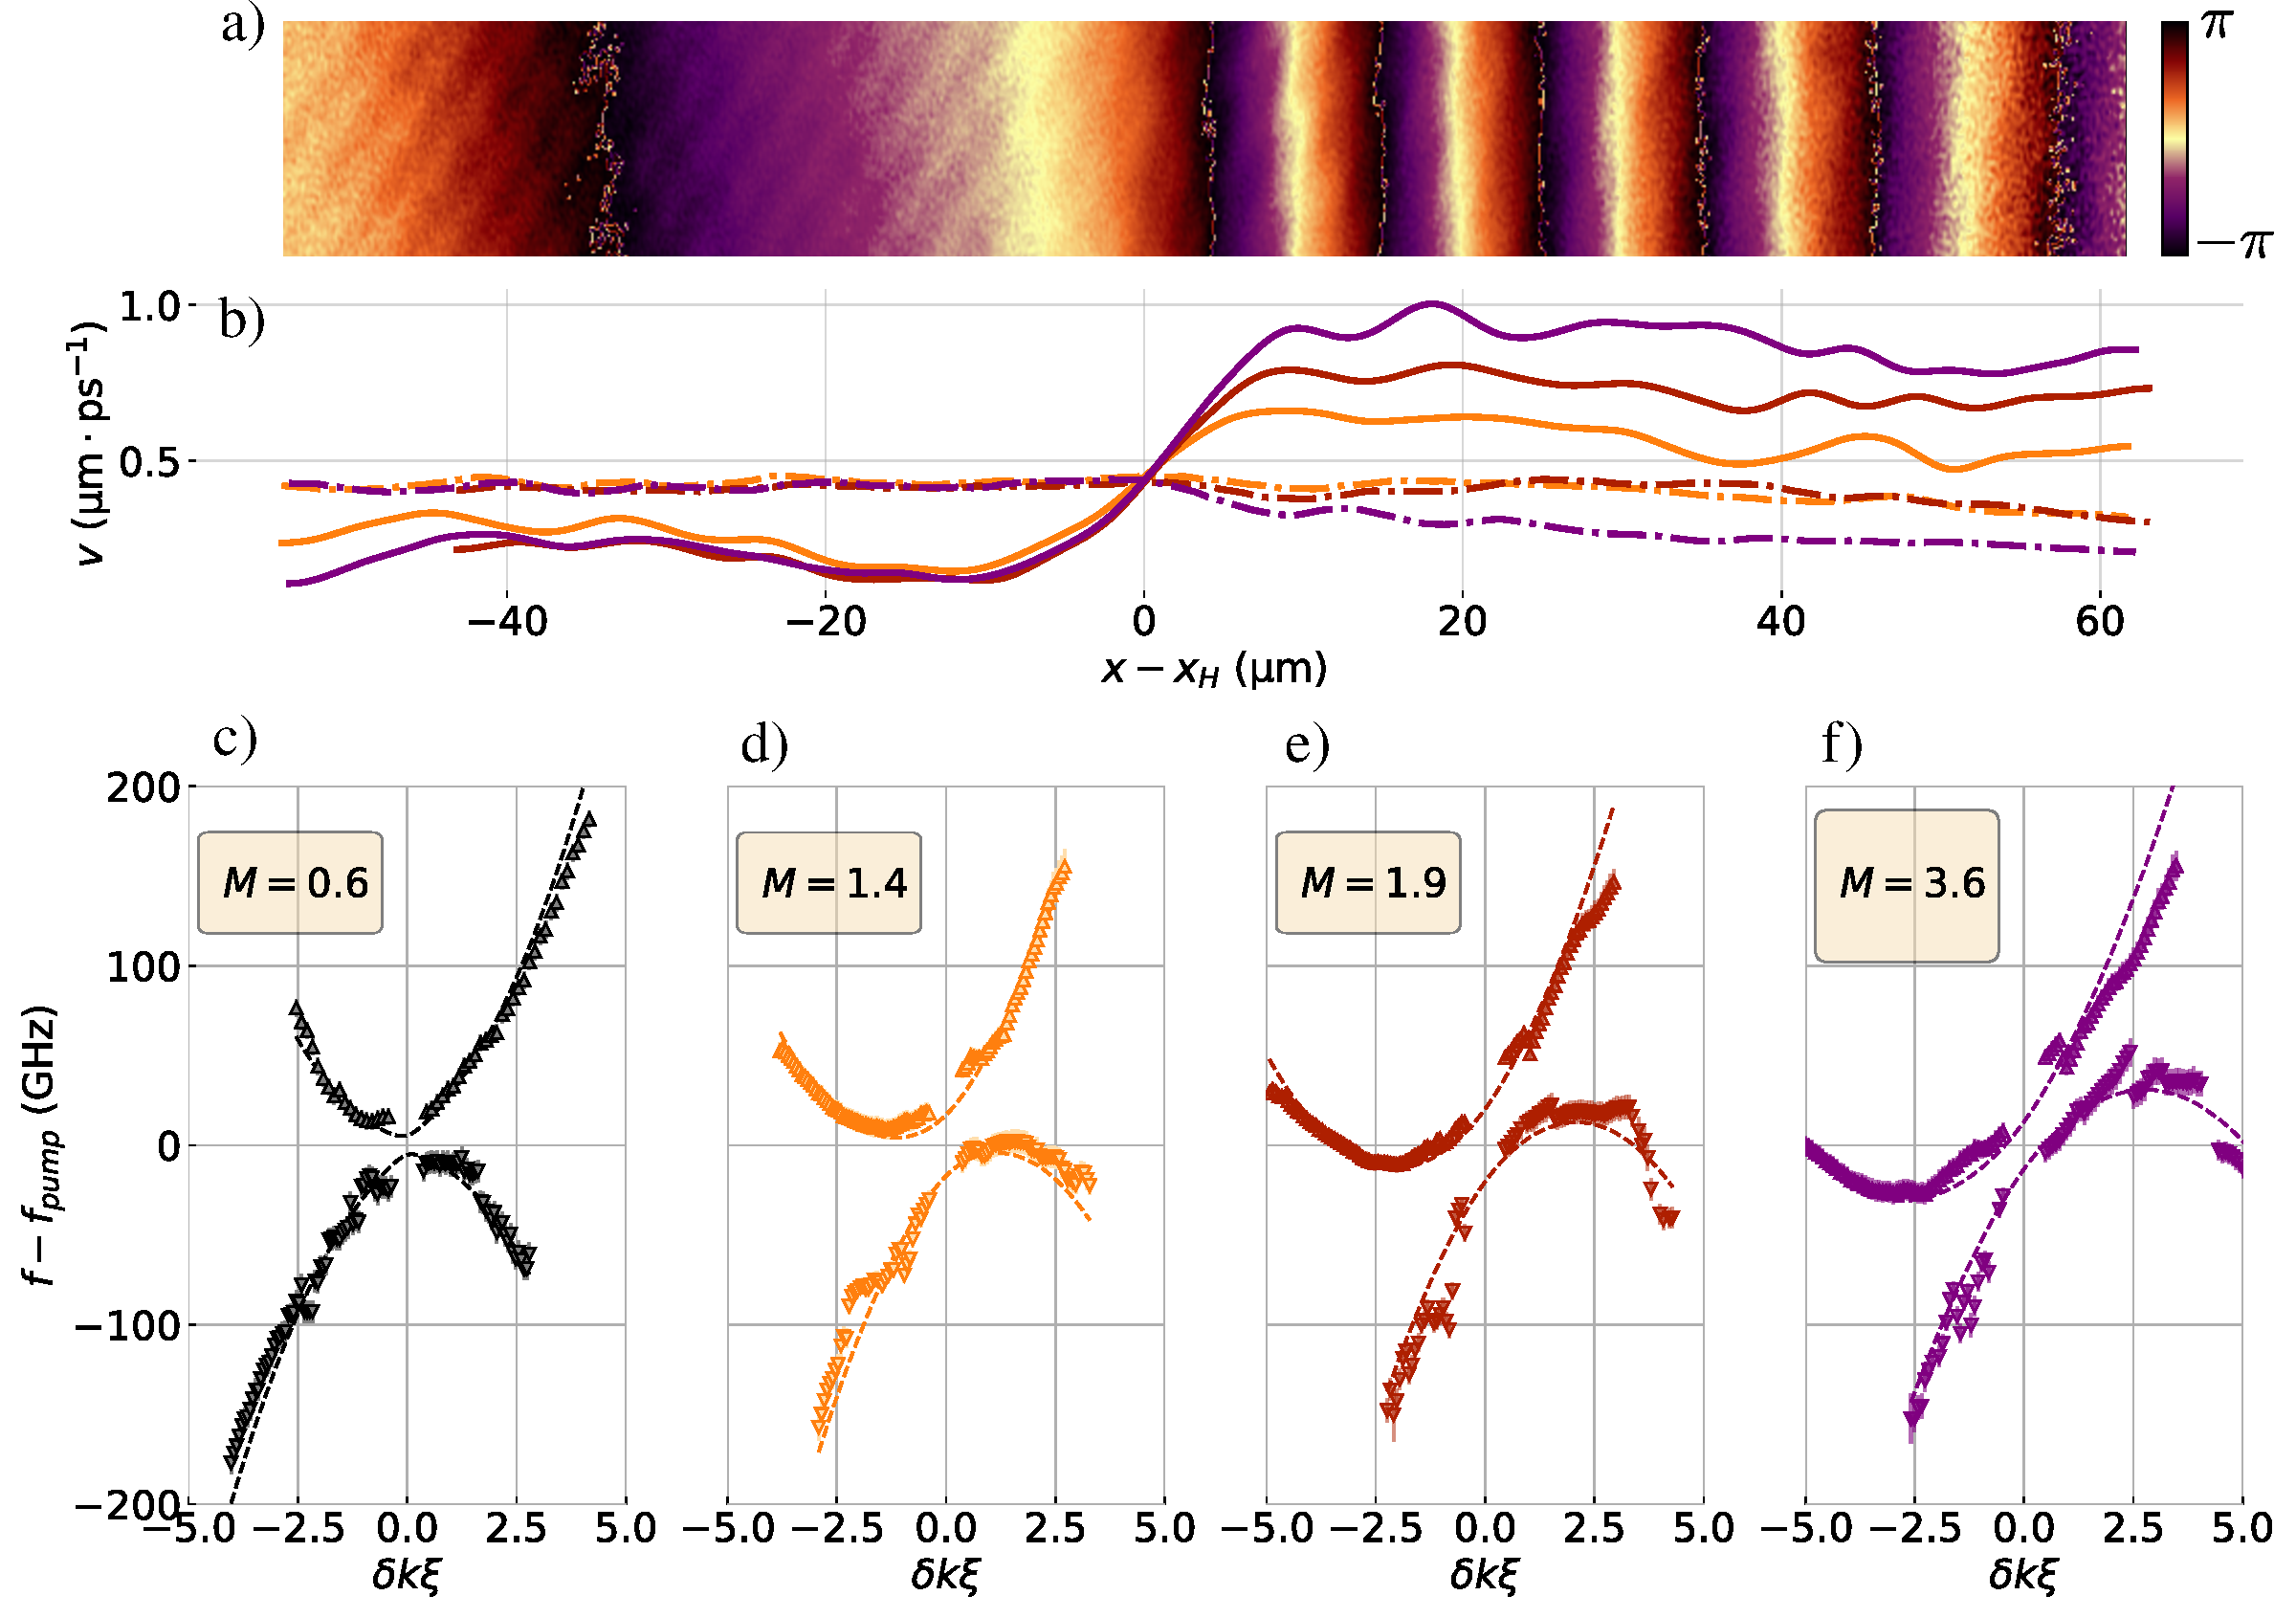
\includegraphics[width=1\textwidth]{chap_custom_st/fig/bh_smooth.pdf}
    \caption{\textbf{Smooth horizon}.
    \textbf{a)} Typical measured phase of the fluid $\theta(x)$ inside the region of interest as defined in \autoref{fig:phase_example}.
    \textbf{\textbf{b)}} Fluid velocity profiles.
    Solid lines, $v_0(x)$; dot-dashed lines, $c_\mathrm{s}(x)$. Orange, $M_\mathrm{u}=0.6$ and $M_\mathrm{d}=1.4$; red, $M_\mathrm{u}=0.4$ and $M_\mathrm{d}=1.9$; purple $M_\mathrm{u}=0.5$ and $M_\mathrm{d}=3.6$.
    \textbf{Excitation spectra} Eq.~\eqref{eq:lfbogo}: \textbf{c)} typical upstream region; \textbf{d)}-\textbf{f)} downstream region.
    Up-triangles, positive-norm branch $\omega_\mathrm{B}^+$; down-triangles, negative-norm branch $\omega_\mathrm{B}^-$; dashed lines, fit with free parameter $gn$. Error bars mostly come from the uncertainty in the determination
    of the center of the lorentzian function used to fit each scan.
    \label{fig:smooth_transition}}
\end{figure}




\subsubsection{Critical velocity} In conservative fluids, sub- and supercritical flows are discriminated by the Mach number $M\coloneqq v_0/c_\mathrm{s}=1$.
Instead, in our driven-dissipative fluid, the minimum velocity to have a supercritical dispersion is larger than $c_\mathrm{s}$.
As a result, the condition $M=1$, which defines the acoustic horizon in the hydrodynamic limit does not necessarily coincide with the condition to excite negative energy waves in the system. In other words the position at 
which the velocities exceed $c_\mathrm{s}$ in \autoref{fig:smooth_transition} \textbf{b)} does not define the horizon of the fluid. Indeed, when the system does not operate at the turning
point of the bistability we have $gn>\delta(k_p)-g_rn_r$, which opens a gap in the dispersion. We rewrite the dispersion in the laboratory frame in a form that allows to easily identify the effect of the gap on the spectrum,


\begin{align}\label{eq:lfbogom}
    \omega^\pm_\mathrm{B}(\delta k)=&v_0(x) ,\delta k(x)-i\frac{\gamma}{2}\nonumber\pm\Biggl[\left(\frac{\hbar\delta k(x)^2}{2 \mlp}\right)^2+\frac{\hbar \delta k(x)^2}{\mlp}(2g n_0 - \delta(k_\mathrm{p})+g_\mathrm{r}n_\mathrm{r})\\
    &\,\,+(g n_0 - \delta(k_\mathrm{p})+g_\mathrm{r}n_\mathrm{r})(3 g n_0 - \delta(k_\mathrm{p})+g_\mathrm{r}n_\mathrm{r})\Biggr]^{-1/2}\nonumber\\
    =&v_0(x) \delta k(x)-i\frac{\gamma}{2}\,\pm\sqrt{\left(\frac{\hbar\delta k(x)^2}{2 \mlp}\right)^2+c_\mathrm{B}^2\delta k(x)^2+\mbogo^2c_\mathrm{B}^4}
\end{align}

where we defined :
\begin{subequations}
    \label{eq:m_bog}
    \begin{align}
    c_B & = \sqrt{\dfrac{\hbar(2gn_0- \delta(k_p)+g_\mathrm{r}n_\mathrm{r})}{\mlp}},\\
    \mbogo&=\mlp\dfrac{\sqrt{(gn_0- \delta(k_p)+g_\mathrm{r}n_\mathrm{r})(3gn_0- \delta(k_p)+g_\mathrm{r}n_\mathrm{r})}}{(2gn_0- \delta(k_p)+g_\mathrm{r}n_\mathrm{r})}.
    \end{align}
\end{subequations}

These two quantities have a well defined physical meaning as follows. 
On the one hand, $\mbogo c_\mathrm{B}^2$ is the energy of $k=0$ modes of $\phi$, introducing a mass gap which vanishes when the system operates at the turning point of the bistability.
On the other hand, ?? is a hyperbolic PDE whose characteristic curves in a fluid at rest are given by $|\pmb{x}|=c_\mathrm{B} t$. These characteristic curves  limit the speed at which the excitations $\phi$ can propagate information, defining the sound cones in full analogy to light cones. However, due to the mass gap, the speed of propagation of excitations of $\phi$ is $v_{\rm g}=d\omega/dk\leq c_\mathrm{B}$. 
The latter can be seen as the limiting speed of propagation of $k\to\infty$ perturbations. This is also in full analogy to propagation of modes of a massive relativistic scalar field, which travel at subluminal speeds, reaching only the speed of light in the limit of infinite momentum.
From \autoref{eq:lfbogom} we see that the field mass $\mbogo$ increases $\abs{\mathrm{Re}(\omega_\mathrm{B}^{\prime\pm})}$ at all $k$, meaning that the critical velocity to have a Doppler effect large enough to excite negative energy  waves is larger than $c_s$.
The value of the critical velocity $v_c=\hbar k_c/\mlp$ at which negative energy waves become available at positive frequency can be computed as follows. 


For $k_p>k_c$, there will be negative norm modes available at positive frequencies, and there will be two values $\delta k_{1,2}$ at which each dispersion branch intersects the horizontal axes. These $\delta k_{1,2}$ depend on the value of $k_p, gn$ and $g_rn_r$. 
The critical wavenumber $k_c$, and correspondingly the critical velocity $v_c=\hbar k_c/\mlp$, is obtained when the two intersection points merge, so that $\delta k_1=\delta k_2=\delta k_0$.
In practice, we compute numerically the  normal branch $\omega_B^+(\delta k)$ spectrum for different values of $k_p$ and $gn$ while keeping the zero momentum detuning constant 
and equal to $\delta(0)=\SI{56}{\giga\hertz}$ as in the experiment. On each computed spectrum, we verify if it exhibits negative frequency values. We obtain the map shown in \autoref{fig:critical_velocity_map}, indicating  if a fluid with given velocity and interaction energy is super-critical. The points c), d), e) and f) correspond to the measured spectrum of \autoref{fig:smooth_transition}.
As it can be seen, the upstream region and downstream region with the smaller velocity do not lie in the super-critical regime whereas e) and f) do. This is in agreement with the fact that the critical velocity is larger than the speed of sound since 
all the regime yielding super-critical flows are located on the right side of the black dashed line corresponding to the acoustic case $c_s = \hbar k_p/\mlp=\sqrt{\hbar gn/\mlp}$. Moreover, the map predicts that configuration d) is subcritical despite a 
Mach number $M_d=1.34$ greater than one.

\bigskip

\textbf{Cutoff spatial frequency.} The absence of experimental data points at wavevectors $\delta k < 0.10 \mu m^{-1}$ is a consequence of the finite size 
of the probe beam $\delta_x = \SI{60}{\micro\meter}$ which fixes the spatial extension of the probe in momentum space
 scaling as $2\pi/\delta_x=0.10 \mu m^{-1}$. At very small wavevector, the probe and its conjugated counterpart start to overlap and photons
 coming from both branches are collected by the pinhole. This prevent the effective discrimination between the two modes in the ouput signal of the photodiode. In practive the 
 cutoff frequency is computed by a simple optical Rayleigh criterion stating that two points are resolved if the distance between them is larger than the FWHM of the point spread function.
In our case this directly gives $\delta k_{cut} = 2\pi/\delta_x= 0.10 \mu m^{-1}$.

\begin{figure}
    \centering
    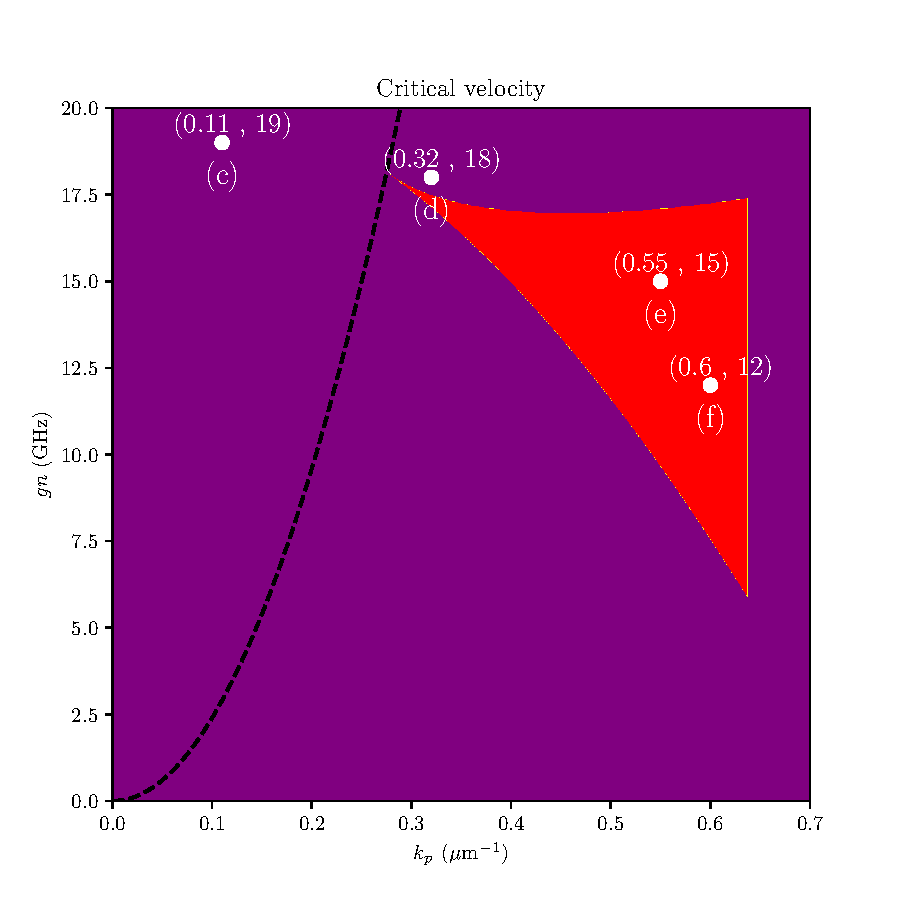
\includegraphics[width=0.8\textwidth]{chap_custom_st/fig/critical_velocity_map.pdf}
    \caption{Critical velocity map as a function of $k_p$ and $gn$ while the reservoir contribution was fixed as $g_rn_r\approx 1.8=gn$. For each couple $(k_p,gn)$ the Bogoliubov spectrum \autoref{eq:lfbogo} is computed : red points correspond to super critical flows and purple point to sub-critical flows.
    The points c), d), e) and f) correspond to the measured spectrum of \autoref{fig:smooth_transition}. The black dashed line represent the acoustic case where the critical velocity coincides with the speed of sound $c_s = \hbar k_s/\mlp=\sqrt{\hbar gn/\mlp}$ }
    \label{fig:critical_velocity_map}
\end{figure}

\subsubsection{Paired emission frequency range}

The paired emission of correlated mode at the horizon requires the mixing of positive and negative energy modes. Consequently the finite velocity in the downstream region 
sets a maximum frequency at which the effect can occur \cite{jacquet_hawking_2019}. This frequency is given by the maximum energy of the negative energy modes that can be excited in the downstream region and is ultimately 
set by the asymptotic downstream velocity $v_d$ and the interaction energy $gn$. Increasing this range result in a larger number of correlated pairs emitted and is expected to enhanced
the overall correlation signal \cite{jacquet_hawking_2019}. 
In \autoref{fig:hawking_range} we plot the analitycal Bogoliubov dispersion corresponding to the measurement of \autoref{fig:smooth_transition} c), e) and f).  Paired emission is then possible in the red range of \autoref{fig:hawking_range}  where negative energy modes
can mix with the positive energy mode of the upstream spectrum, located outside the gap represented in blue.

The overall frequency range at which Hawking emission is possible is given by :

\begin{equation}
    \begin{align}
    \Delta \omega_H& \coloneqq  2\omega_{max}- \Delta\omega_{gap}
    \end{align}  
    \label{eq:hawking_range}
\end{equation}

where $\omega_{max}$ is the maximum energy of the negative energy modes that can be excited in the downstream region and $\Delta\omega_{gap}$ the width 
of the gap in the upstream spectrum. We measure $\Delta \omega_H$=6 GHz for the e) configuration and 30 GHz for the fastest flow. 
Hence by changing the asymptotic downstream speed our system enables to tune the number of states available for paired emission. Let us now 
show that we can control another crucial parameter of the Hawking radiation, the steepness of the horizon.

\begin{figure}
    \centering
    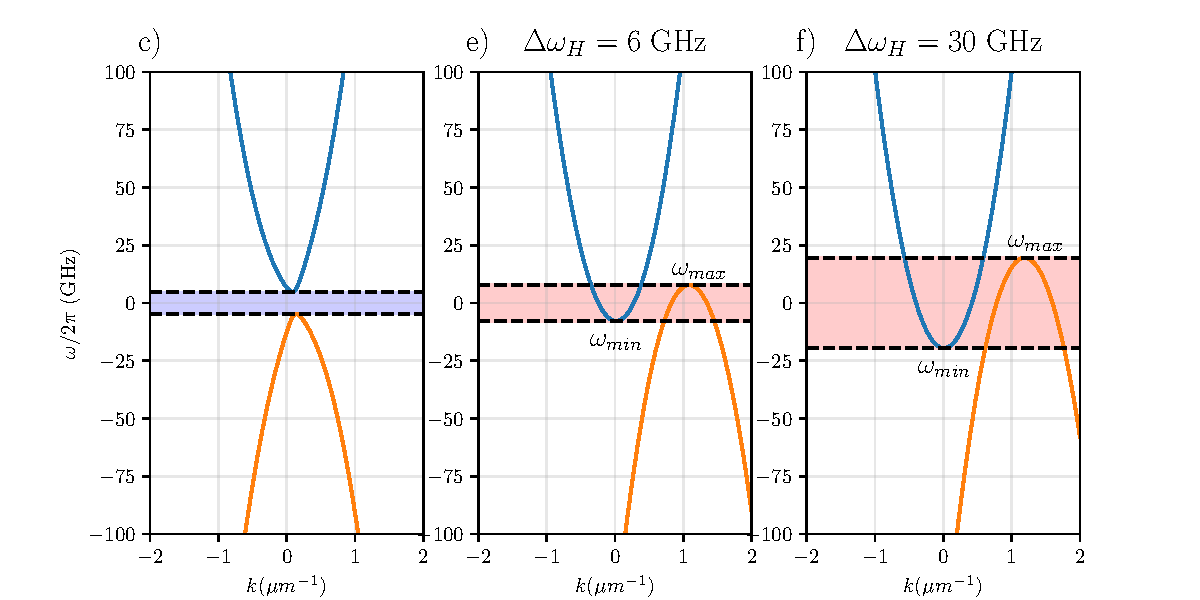
\includegraphics[width=0.8\textwidth]{chap_custom_st/fig/max_freq_hawking.pdf}
    \caption{c) , e) , f) analytical Bogoliubov dispersion corresponding to the fit of \autoref{fig:smooth_transition} c), e) and f). The red range in e) and f) represents the frequency range at which negative energy modes
    are available that can mix with the positive energy modes outside the gap represented in blue whose value $\Delta \omega_H$ are displayed above each plot.}
    \label{fig:hawking_range}
\end{figure}

\subsection{Steep horizon geometry}

The sharpness of the transition is a crucial parameter to study the strength of correlation of the emitted modes. It can be evaluated with the following equation :
\begin{equation}
    \kappa \coloneqq \frac{1}{2c_\mathrm{s}(x)}\frac{d}{dx}[v^2_0(x)-c^2_\mathrm{s}(x)]|_{x_\mathrm{H}},
    \label{eq:steepness}
\end{equation}
the hydrodynamic equivalent to surface gravity \cite{barcelo_hawking-like_2006}. However the discussion in the previous section 
pointed out that the position $x_H$ at which the fluid velocity exceed the speed of sound does not define the horizon of the fluid, the derivative
in the definition of $\kappa$ should then be taken at the position where the critical velocity is reached and involves the critical velocity instead of $c_s$.
In practice this brings only a negligible correction to the value of $\kappa$. 

\bigskip

\textbf{Increasing the surface gravity.}
The steepness of the horizon can be tuned in two ways. First, by reducing the width of the transition $w_H$ in the target velocity profile.
Second, by taking advantage of the dependence of the bistability cycle on the effective detuning $\delta(k_p)$.
As shown in \autoref{fig:optical_bistability} \textbf{b)} the value of $gn$ with a fixed input intensity increases linearly with the effective detuning until the turning point is reached. More precisely,
when the pump wavevector is increased,  $\delta(k_p) = \omega_p-\omega_{LP}^{(0)}- \hbar k_p^2/2\mlp$ decreases and so does $gn$ as shown in \autoref{fig:bistab_steep}. In some
sense the microcavity naturally reduce the density of the fluid when the pump wavevector is increased, moving the laser away from resonance.
In practice, we tune wisely the energy of the pump laser and the asymptotic upstream and downstream target wavevevectors. The different values of $\delta(k_{up})$ and $\delta(k_{d})$ can
lead to region with different $gn$ values as shown on \autoref{fig:bistab_steep}.
Here we create a trans critical flow with a sharper transition in order to increase the value 

\begin{figure}
    \centering
    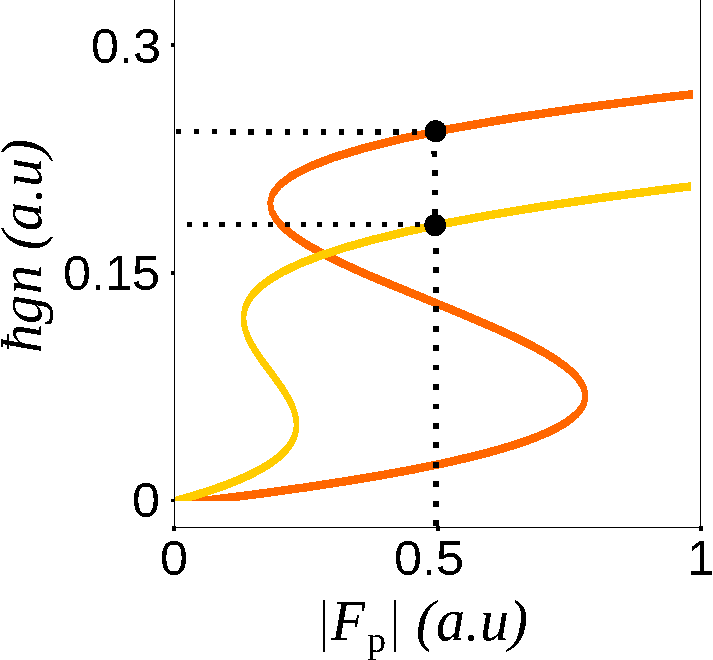
\includegraphics[width=0.4\textwidth]{chap_custom_st/fig/bistab_to_gn.pdf}
    \caption{Bistability cycle for two different values of the effective detuning $\delta(k^{(1)}_p)$ (yellow) $\leq \delta(k^{(2)}_p) $ (orange) when $k^{(2)}_p \leq k^{(1)}_p $. The vertical dashed line
    represents the input intensity of the pump laser whereas the black dots represent the operating points of the system for each detuning. The region with the higher wavevector
    yields a lower $gn$ value.}
    \label{fig:bistab_steep}
\end{figure}

Here we exploit the phenomenology and implement the target profile \autoref{eq:target_velocity} with a large difference between $v_\mathrm{d}$ and $v_\mathrm{u}$, a transition width $w_\mathrm{H}=\SI{20}{\micro\meter}$ and a detuning $\delta(0)=\SI{71}{\giga\hertz} \rightarrow\hbar\delta(0)=\SI{0.3}{\milli \electronvolt}$
\autoref{fig:bh_steep} (\textbf{b)} shows $v_0(x)$ (solid lines) as well as $c_\mathrm{s}(x)$ (dot-dashed lines). The two supercritical fluids created in the smooth configuration 
have an horizon steepness $\kappa$ of $\SI{0.07}{\per \pico \second}$ (red) and $\SI{0.08}{\per \pico \second}$ (purple) whereas in the steep geometry implemented here we compute $\kappa = \SI{0.11}{\per \pico \second}$. The excitation spectra are shown in \autoref{fig:bh_steep} \textbf{c)} and \textbf{d)}.
The frequency range at which paired emission is possible is roughly the same than in the smooth case \textbf{f)} $\Delta \omega_H$= 28 GHz whereas the horizon steepness 
gets increased by 25\%. This independent tuning of $\kappa$ and the paired emission spectrum is not possible in conservative quantum fluids such as atomic BECs, for example.
The fine control over the waterfall horizon geometry we demonstrate here is interesting to test recent tunneling models for the Hawking effect~\cite{delporro2024tunneling}.


\begin{figure}
    \centering
    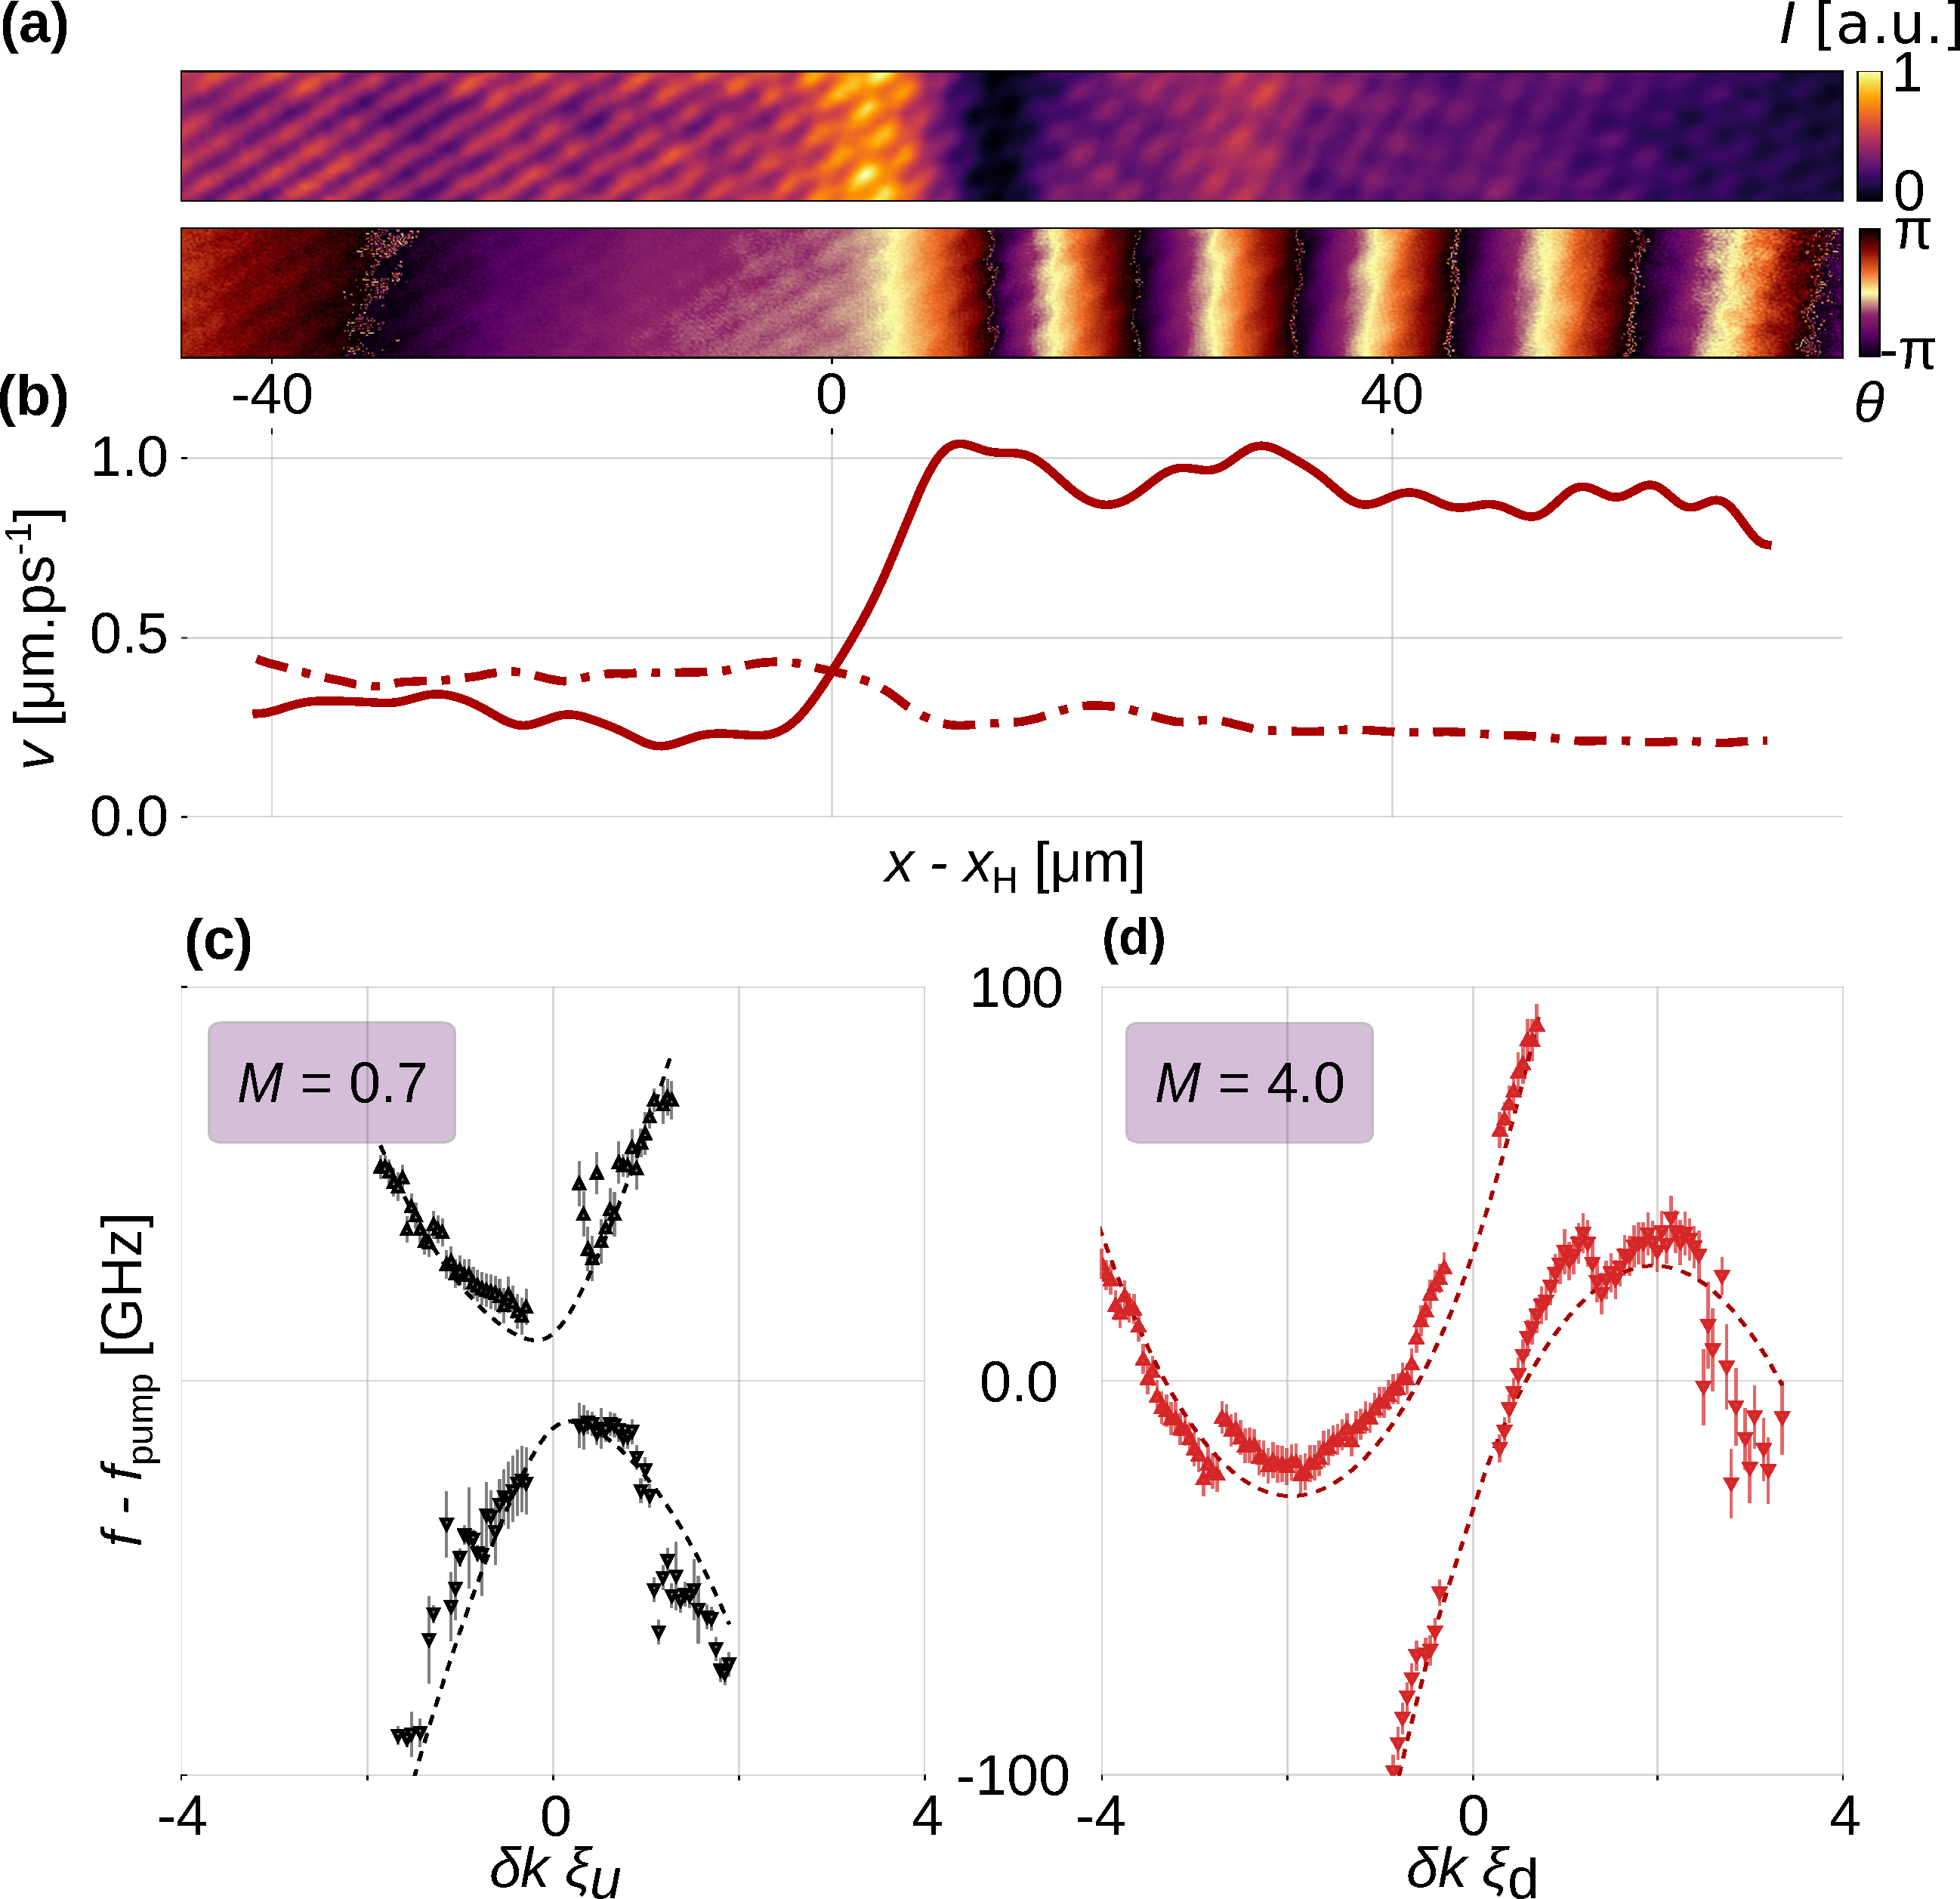
\includegraphics[width=0.7\textwidth]{chap_custom_st/fig/bh_steep.pdf}
    \caption{\textbf{Steep horizon}.    
    \textbf{(a)} Measured fluid density (top) and phase (bottom).
    \textbf{(b)} Measured fluid velocity profile.
    Solid line, $v_0(x)$; dashed line, $c_\mathrm{s}(x)$.
    \textbf{Excitation spectra} Eq.~\eqref{eq:lfbogo}: \textbf{(c)} upstream region. \textbf{(d)} downstream region; dashed lines, fit with free parameter $gn$. Error bars represent the uncertainty in the determination
    of the center of the lorentzian when each scan is fitted by a lorentzian function to find the resonance energy. The $M$ values in the inset of each spectrum is the computed Mach number in the corresponding region. }
    \label{fig:bh_steep}
\end{figure}

\subsection{Quasi-normal mode configuration}

The target velocity profile \autoref{eq:target_velocity} can be modified to create complex horizon geometry by imprinting 
a velocity peak in the transition region. More precisely, we define the \textit{Quasi-Normal Mode} (QNM) target velocity profile as :

\begin{figure}
    \centering
    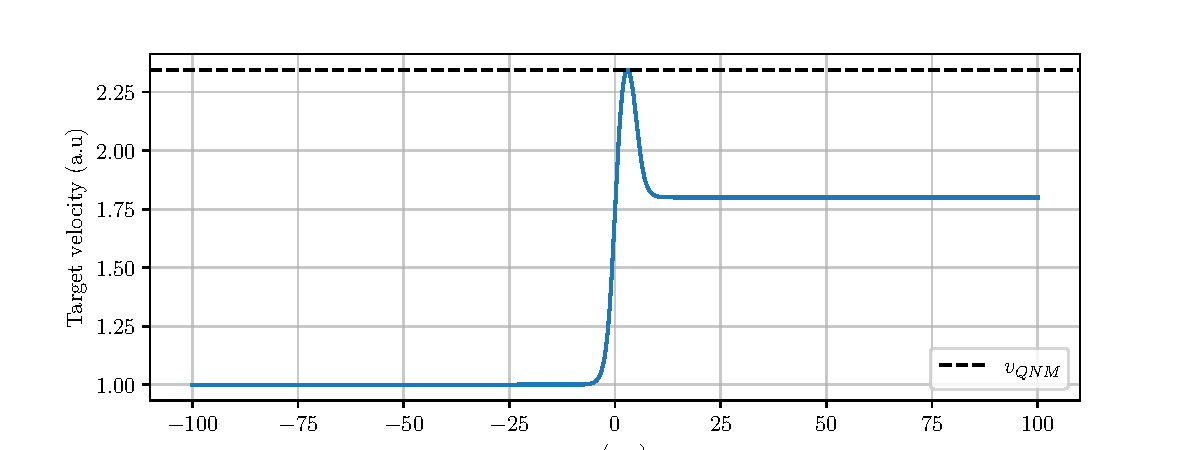
\includegraphics[width=1\textwidth]{chap_custom_st/fig/qnm_target_velocity.pdf}
    \caption{Typical QNM target velocity profile.}
    \label{fig:qnm_target_velocity}
\end{figure}


\begin{equation}
    v(x)= \frac{v_{QNM}-v_{up}}{2}\mathrm{tanh}(\frac{x-x_1}{w_1})+ \frac{v_{d}-v_{QNM}}{2}\mathrm{tanh}(\frac{x-x_2}{w_2})+\frac{v_{up}+v_{d}}{2}
    \label{eq:target_velocity_qnm}
\end{equation}

where $v_{QNM}$ is the velocity of the peak, $v_{up}$ and $v_{d}$ are the upstream and downstream velocities, $x_1$ and $x_2$ are the position of the first and second transition and $w_1$ and $w_2$ are their width.
The typical corresponding shape is shown in \autoref{fig:qnm_target_velocity}.
With the same asymptotic parameters as in the smooth horizon configuration of \autoref{fig:smooth_transition} \textbf{e)} we create a fluid with the QNM target velocity profile.
\begin{figure}
    \centering
    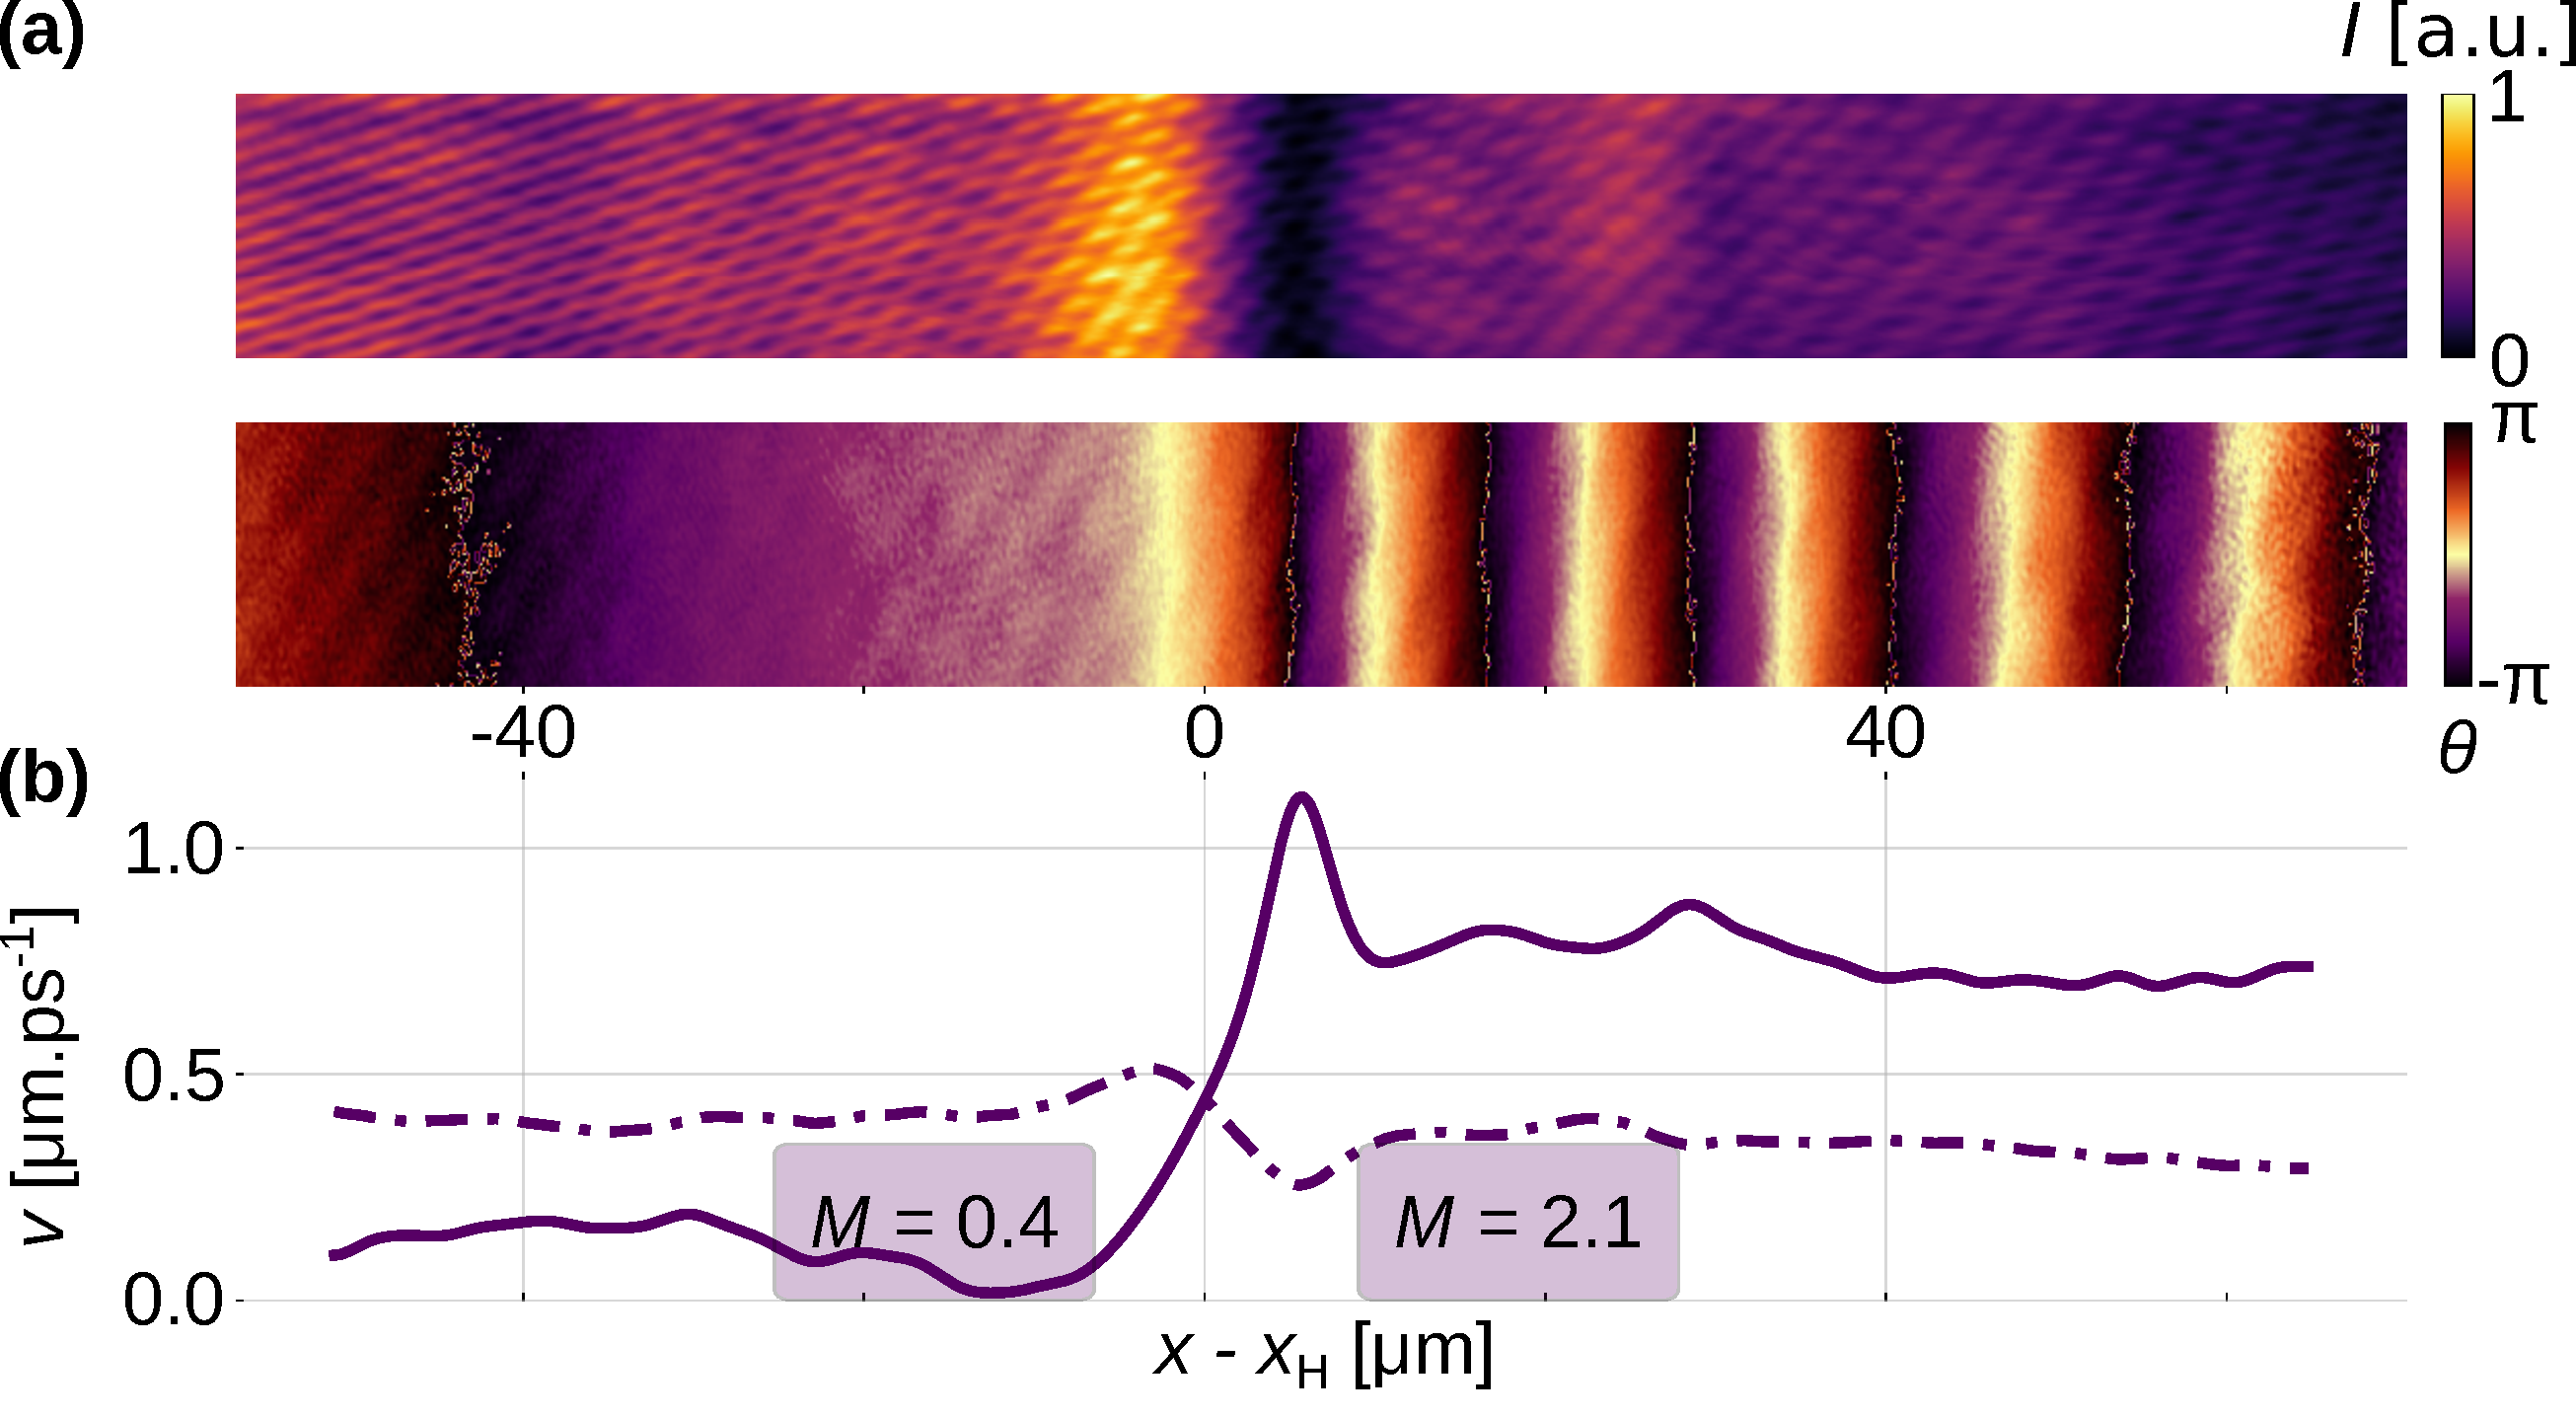
\includegraphics[width=0.7\textwidth]{chap_custom_st/fig/bh_qnm.pdf}
    \caption{\textbf{Quasi-normal mode horizon}.    
    \textbf{(a)} Measured fluid density (top) and phase (bottom).
    \textbf{(b)} Measured fluid velocity profile.
    Solid line, $v_0(x)$; dashed line, $c_\mathrm{s}(x)$.}
    \label{fig:bh_qnm}
\end{figure}

First, the asymptotic velocities are as expected, not modified by the presence of the peak, while the surface gravity 
is greatly enhanced as $\kappa = \SI{0.19}{\per \pico \second}$, almost twice the value obtained in the steep configuration.
But the most peculiar feature of the QNM configuration is the density dip that comes with the velocity peak. For the reason explained in the previous section,
the velocity peak imprinted here is associated with a density dip. As the dip is surrounded by two regions of higher density, it forms an effective resonator for Bogoliubov excitation.
This leads to the appearance of a metastable excitation mode of $\phi$ called a quasi-normal mode: here specifically, a negative-energy standing wave can establish itself inside the resonator (at $\omega_\mathrm{QNM}>\mathrm{max}(\omega_\mathrm{B}^-|_{x>x_\mathrm{H}})$) and tunnel-couple with positive-energy propagating waves on either side \cite{jacquet_quantum_2023}.
This quasi-normal mode is spontaneously excited by quantum vacuum fluctuations of $\phi$.
As a result, the Hawking spectrum is predicted to peak at the frequency of the quasi-normal mode, bearing signatures of the near-horizon geometry. 
In some sense, the QNM configuration is a quantum analogue of the black hole ringdown phase, where the black hole emits gravitational waves with a characteristic frequency and damping time \cite{brito_gravitational_2015} that depend on its parameters. 


\section{Conclusion}

We demonstrated full optical generation and characterization of mean field with arbitrary velocity profiles in a polariton fluid which act as an effectively curved spacetime for 
Bogoliubov excitations. In each
configuration, we were able to measure the collective excitations spectrum of the fluid and state or not if Hawking radiation could be observed. We showed that the critical velocity to observe negative energy modes is not necessarily the speed of sound but rather a critical velocity 
that depends on the fluid parameters. This widens the range of experimental configurations at which particle creation can be observed. The great versatility of our experimental methods also showed that the steepness of the horizon can be controlled independently of the paired emission spectrum.
Finally, we demonstrated the possibility to create complex horizon geometry that could yield peculiar behaviors like Quasi Normal Modes. The great 
advantage of the system presented here is the large range of field theory scenarii that can be tested in a single setup. Even though
 trans-critical polariton fluids are far from encapsulating what truly happens at a black hole horizon, its a great platform to study effects predicted by field theory in curved spacetime, regardless they were
originally thought for black holes or not.

\subsection{Outlook}
